% Options for packages loaded elsewhere
\PassOptionsToPackage{unicode}{hyperref}
\PassOptionsToPackage{hyphens}{url}
\PassOptionsToPackage{dvipsnames,svgnames,x11names}{xcolor}
%
\documentclass[
  letterpaper,
  DIV=11,
  numbers=noendperiod]{scrreprt}

\usepackage{amsmath,amssymb}
\usepackage{lmodern}
\usepackage{iftex}
\ifPDFTeX
  \usepackage[T1]{fontenc}
  \usepackage[utf8]{inputenc}
  \usepackage{textcomp} % provide euro and other symbols
\else % if luatex or xetex
  \usepackage{unicode-math}
  \defaultfontfeatures{Scale=MatchLowercase}
  \defaultfontfeatures[\rmfamily]{Ligatures=TeX,Scale=1}
\fi
% Use upquote if available, for straight quotes in verbatim environments
\IfFileExists{upquote.sty}{\usepackage{upquote}}{}
\IfFileExists{microtype.sty}{% use microtype if available
  \usepackage[]{microtype}
  \UseMicrotypeSet[protrusion]{basicmath} % disable protrusion for tt fonts
}{}
\makeatletter
\@ifundefined{KOMAClassName}{% if non-KOMA class
  \IfFileExists{parskip.sty}{%
    \usepackage{parskip}
  }{% else
    \setlength{\parindent}{0pt}
    \setlength{\parskip}{6pt plus 2pt minus 1pt}}
}{% if KOMA class
  \KOMAoptions{parskip=half}}
\makeatother
\usepackage{xcolor}
\setlength{\emergencystretch}{3em} % prevent overfull lines
\setcounter{secnumdepth}{5}
% Make \paragraph and \subparagraph free-standing
\ifx\paragraph\undefined\else
  \let\oldparagraph\paragraph
  \renewcommand{\paragraph}[1]{\oldparagraph{#1}\mbox{}}
\fi
\ifx\subparagraph\undefined\else
  \let\oldsubparagraph\subparagraph
  \renewcommand{\subparagraph}[1]{\oldsubparagraph{#1}\mbox{}}
\fi


\providecommand{\tightlist}{%
  \setlength{\itemsep}{0pt}\setlength{\parskip}{0pt}}\usepackage{longtable,booktabs,array}
\usepackage{calc} % for calculating minipage widths
% Correct order of tables after \paragraph or \subparagraph
\usepackage{etoolbox}
\makeatletter
\patchcmd\longtable{\par}{\if@noskipsec\mbox{}\fi\par}{}{}
\makeatother
% Allow footnotes in longtable head/foot
\IfFileExists{footnotehyper.sty}{\usepackage{footnotehyper}}{\usepackage{footnote}}
\makesavenoteenv{longtable}
\usepackage{graphicx}
\makeatletter
\def\maxwidth{\ifdim\Gin@nat@width>\linewidth\linewidth\else\Gin@nat@width\fi}
\def\maxheight{\ifdim\Gin@nat@height>\textheight\textheight\else\Gin@nat@height\fi}
\makeatother
% Scale images if necessary, so that they will not overflow the page
% margins by default, and it is still possible to overwrite the defaults
% using explicit options in \includegraphics[width, height, ...]{}
\setkeys{Gin}{width=\maxwidth,height=\maxheight,keepaspectratio}
% Set default figure placement to htbp
\makeatletter
\def\fps@figure{htbp}
\makeatother
\newlength{\cslhangindent}
\setlength{\cslhangindent}{1.5em}
\newlength{\csllabelwidth}
\setlength{\csllabelwidth}{3em}
\newlength{\cslentryspacingunit} % times entry-spacing
\setlength{\cslentryspacingunit}{\parskip}
\newenvironment{CSLReferences}[2] % #1 hanging-ident, #2 entry spacing
 {% don't indent paragraphs
  \setlength{\parindent}{0pt}
  % turn on hanging indent if param 1 is 1
  \ifodd #1
  \let\oldpar\par
  \def\par{\hangindent=\cslhangindent\oldpar}
  \fi
  % set entry spacing
  \setlength{\parskip}{#2\cslentryspacingunit}
 }%
 {}
\usepackage{calc}
\newcommand{\CSLBlock}[1]{#1\hfill\break}
\newcommand{\CSLLeftMargin}[1]{\parbox[t]{\csllabelwidth}{#1}}
\newcommand{\CSLRightInline}[1]{\parbox[t]{\linewidth - \csllabelwidth}{#1}\break}
\newcommand{\CSLIndent}[1]{\hspace{\cslhangindent}#1}

\KOMAoption{captions}{tableheading}
\makeatletter
\@ifpackageloaded{tcolorbox}{}{\usepackage[many]{tcolorbox}}
\@ifpackageloaded{fontawesome5}{}{\usepackage{fontawesome5}}
\definecolor{quarto-callout-color}{HTML}{909090}
\definecolor{quarto-callout-note-color}{HTML}{0758E5}
\definecolor{quarto-callout-important-color}{HTML}{CC1914}
\definecolor{quarto-callout-warning-color}{HTML}{EB9113}
\definecolor{quarto-callout-tip-color}{HTML}{00A047}
\definecolor{quarto-callout-caution-color}{HTML}{FC5300}
\definecolor{quarto-callout-color-frame}{HTML}{acacac}
\definecolor{quarto-callout-note-color-frame}{HTML}{4582ec}
\definecolor{quarto-callout-important-color-frame}{HTML}{d9534f}
\definecolor{quarto-callout-warning-color-frame}{HTML}{f0ad4e}
\definecolor{quarto-callout-tip-color-frame}{HTML}{02b875}
\definecolor{quarto-callout-caution-color-frame}{HTML}{fd7e14}
\makeatother
\makeatletter
\makeatother
\makeatletter
\@ifpackageloaded{bookmark}{}{\usepackage{bookmark}}
\makeatother
\makeatletter
\@ifpackageloaded{caption}{}{\usepackage{caption}}
\AtBeginDocument{%
\ifdefined\contentsname
  \renewcommand*\contentsname{Table of contents}
\else
  \newcommand\contentsname{Table of contents}
\fi
\ifdefined\listfigurename
  \renewcommand*\listfigurename{List of Figures}
\else
  \newcommand\listfigurename{List of Figures}
\fi
\ifdefined\listtablename
  \renewcommand*\listtablename{List of Tables}
\else
  \newcommand\listtablename{List of Tables}
\fi
\ifdefined\figurename
  \renewcommand*\figurename{Figure}
\else
  \newcommand\figurename{Figure}
\fi
\ifdefined\tablename
  \renewcommand*\tablename{Table}
\else
  \newcommand\tablename{Table}
\fi
}
\@ifpackageloaded{float}{}{\usepackage{float}}
\floatstyle{ruled}
\@ifundefined{c@chapter}{\newfloat{codelisting}{h}{lop}}{\newfloat{codelisting}{h}{lop}[chapter]}
\floatname{codelisting}{Listing}
\newcommand*\listoflistings{\listof{codelisting}{List of Listings}}
\makeatother
\makeatletter
\@ifpackageloaded{caption}{}{\usepackage{caption}}
\@ifpackageloaded{subcaption}{}{\usepackage{subcaption}}
\makeatother
\makeatletter
\@ifpackageloaded{tcolorbox}{}{\usepackage[many]{tcolorbox}}
\makeatother
\makeatletter
\@ifundefined{shadecolor}{\definecolor{shadecolor}{rgb}{.97, .97, .97}}
\makeatother
\makeatletter
\makeatother
\makeatletter
\@ifpackageloaded{fontawesome5}{}{\usepackage{fontawesome5}}
\makeatother
\ifLuaTeX
  \usepackage{selnolig}  % disable illegal ligatures
\fi
\IfFileExists{bookmark.sty}{\usepackage{bookmark}}{\usepackage{hyperref}}
\IfFileExists{xurl.sty}{\usepackage{xurl}}{} % add URL line breaks if available
\urlstyle{same} % disable monospaced font for URLs
\hypersetup{
  pdftitle={Guide to N3C},
  colorlinks=true,
  linkcolor={blue},
  filecolor={Maroon},
  citecolor={Blue},
  urlcolor={Blue},
  pdfcreator={LaTeX via pandoc}}

\title{Guide to N3C}
\author{}
\date{3/14/23}

\begin{document}
\maketitle
\ifdefined\Shaded\renewenvironment{Shaded}{\begin{tcolorbox}[interior hidden, borderline west={3pt}{0pt}{shadecolor}, sharp corners, boxrule=0pt, frame hidden, enhanced, breakable]}{\end{tcolorbox}}\fi

\renewcommand*\contentsname{Table of contents}
{
\hypersetup{linkcolor=}
\setcounter{tocdepth}{2}
\tableofcontents
}
\bookmarksetup{startatroot}

\hypertarget{welcome}{%
\chapter*{Welcome}\label{welcome}}
\addcontentsline{toc}{chapter}{Welcome}

\markboth{Welcome}{Welcome}

\emph{\href{https://national-covid-cohort-collaborative.github.io/guide-to-n3c-v1/}{The
Guide to N3C}} is designed to guide research with the
\href{https://ncats.nih.gov/n3c}{National COVID Cohort Collaborative}
(N3C).

\hypertarget{contributing-content}{%
\section*{Contributing Content}\label{contributing-content}}
\addcontentsline{toc}{section}{Contributing Content}

\markright{Contributing Content}

The N3C and its \href{https://covid.cd2h.org/domain-teams}{domain teams}
are healthiest when assimilating contributions from reseachers of
different skills (\emph{e.g.}, clinicians \& informaticians),
specialties (\emph{e.g.}, endocrinology \& gerontology), programming
languages (\emph{e.g.}, Python, R, \& SQL) and experiences (\emph{e.g.},
students \& PIs).

Accordingly, the
\href{https://github.com/National-COVID-Cohort-Collaborative/guide-to-n3c-v1}{guide-to-n3c-v1}
repository welcomes input from you.

If you see a small mistake or unclear language, we invite you to inform
us in a
\href{https://github.com/National-COVID-Cohort-Collaborative/guide-to-n3c-v1/issues}{new
issue} or to edit the source and submitting a
\href{https://docs.github.com/en/github/collaborating-with-pull-requests/proposing-changes-to-your-work-with-pull-requests/about-pull-requests}{pull
request}. When an editor reviews and accepts your change, the website
will be updated within minutes.

If you have an idea for something more substantial such as a chapter or
section, please start a
\href{https://github.com/National-COVID-Cohort-Collaborative/guide-to-n3c-v1/issues}{new
issue} and the N3C Educational Committee will coordinate with you where
it fits best.

\hypertarget{platform}{%
\section*{Platform}\label{platform}}
\addcontentsline{toc}{section}{Platform}

\markright{Platform}

As the chapters are being written, talk to the chapter's Lead Author to
learn if it's being written in GitHub or Google Docs. Eventually all
Google Docs chapters will be translated to Markdown. Once a chapter has
been finally converted to Markdown\ldots{}

To make small changes like spelling corrections, we recommend editing
the source directly in GitHub. It handles the details without your
knowledge (like starting a fork and prompting your pull request). From
the appropriate page of
\href{https://national-covid-cohort-collaborative.github.io/guide-to-n3c-v1/}{the
book}, click on the ``Edit this page '' button and type your change in
the
\href{https://docs.github.com/en/repositories/working-with-files/managing-files/editing-files}{GitHub
editor}.

Substantial edits and writing are better accommodated by a text editor
on your local machine that can preview the rendered content as you type.
We suggest \href{https://code.visualstudio.com/}{Visual Studio Code} or
\href{https://www.rstudio.com/products/rstudio/}{RStudio}.

You don't have to understand the rest to contribute, but for those
interested:

\begin{itemize}
\item
  The majority of this book is written in a collection of
  \href{https://guides.github.com/features/mastering-markdown/}{Markdown}
  documents and assembled by the \href{https://quarto.org/}{Quarto}.
\item
  After your change is pushed to GitHub, a
  \href{https://docs.github.com/en/actions/learn-github-actions/understanding-github-actions}{GitHub
  Action} spawns a small VM that (a) collects all the Markdown
  documents, (b) calls
  \href{https://quarto.org/}{Quarto}/\href{https://pandoc.org/}{Pandoc}
  to convert them to html, and (c) moves the rendered html files to the
  ``gh-pages'' branch.
\item
  GitHub Pages serves the contents of the
  \href{https://github.com/National-COVID-Cohort-Collaborative/guide-to-n3c-v1/tree/gh-pages}{\texttt{gh-pages}
  branch} to anyone with a browser.
\end{itemize}

\hypertarget{funding-and-licensing}{%
\section*{Funding and Licensing}\label{funding-and-licensing}}
\addcontentsline{toc}{section}{Funding and Licensing}

\markright{Funding and Licensing}

The N3C is supported by \href{https://www.nih.gov/}{NIH} National Center
for Advancing Translational Sciences
(\href{https://ncats.nih.gov/}{NCATS}).

This book is licensed under the
\href{https://creativecommons.org/licenses/by-nd/4.0/}{Creative Commons
Attribution-NoDerivatives 4.0}. \faIcon{creative-commons}
\faIcon{creative-commons-by} \faIcon{creative-commons-nd}

\part{Getting Started}

\hypertarget{sec-intro}{%
\chapter{Introduction}\label{sec-intro}}

\begin{tcolorbox}[enhanced jigsaw, rightrule=.15mm, colback=white, leftrule=.75mm, breakable, left=2mm, bottomtitle=1mm, opacityback=0, toprule=.15mm, colframe=quarto-callout-note-color-frame, titlerule=0mm, toptitle=1mm, coltitle=black, title=\textcolor{quarto-callout-note-color}{\faInfo}\hspace{0.5em}{Note}, bottomrule=.15mm, arc=.35mm, opacitybacktitle=0.6, colbacktitle=quarto-callout-note-color!10!white]

This chapter is being drafted in Google Docs at
\url{https://drive.google.com/drive/u/0/folders/16QkU2vonX5iZzjsLCxIEREPEdZ9S6wza}

See a draft of the chapter outline at
\url{https://docs.google.com/document/d/1ttUKgwVcIZHM87elrlUNV6Qi9thzOwKBg8GegKObEtg/}

\end{tcolorbox}

\begin{tcolorbox}[enhanced jigsaw, rightrule=.15mm, colback=white, leftrule=.75mm, breakable, left=2mm, bottomtitle=1mm, opacityback=0, toprule=.15mm, colframe=quarto-callout-warning-color-frame, titlerule=0mm, toptitle=1mm, coltitle=black, title=\textcolor{quarto-callout-warning-color}{\faExclamationTriangle}\hspace{0.5em}{Warning}, bottomrule=.15mm, arc=.35mm, opacitybacktitle=0.6, colbacktitle=quarto-callout-warning-color!10!white]

At this point, any edits to this chapter should be made in Google Docs.
The current Markdown is for testing only. It is NOT the source of truth
(yet).

\end{tcolorbox}

\textbf{Additional Contributors:}

\hypertarget{mission}{%
\section{Mission}\label{mission}}

The National COVID Cohort Collaborative, or N3C, is an open-science
community stewarded by the National Center for Data To Health (CD2H) and
the NIH National Center for Advancing Translational Sciences (NCATS),
with significant contributions from many partners including the Clinical
and Translational Science Awards (CTSA) program, Centers for
Translational Research (CTRs), and thousands of researchers from
hundreds of participating institutions in the US and abroad.

Faced with the COVID-19 pandemic, the issue addressed by N3C is clear
and direct: the US has no centralized data repository for health records
and related information, hindering the response of the scientific
community.\footnote{This article in MIT Technology Review provides a
  good overview of N3C and the surrounding landscape:
  \href{https://www.technologyreview.com/2021/06/21/1026590/us-covid-database-n3c-nih-privacy/}{It
  took a pandemic, but the US finally has (some) centralized medical
  data}.} Although healthcare providers are mandated by law to utilize
electronic health records (EHR), little guidance coordinates how or
exactly what information to collect and store. Commercial EHR suites
(e.g.~Epic) are widely used, and controlled vocabularies (e.g.~ICD10 and
SNOMED) provide standards for representing medical information, but
there are many such standards in use and EHR software is highly
configurable to the needs of individual organizations. As a result,
databases of EHR information across the US are largely
non-interoperable, presenting challenges to researchers hoping to use
this vast national store of information in practice.

\hypertarget{common-data-models-and-n3c}{%
\section{Common Data Models and N3C}\label{common-data-models-and-n3c}}

In recent years, the common solution to these issues have been the
creation of \emph{Common Data Models} (CDMs). A Common Data Model is an
agreed-upon structure and format for databases containing clinical
information, into which diverse organizational EHR databases can be
standardized for research purposes. Even so, healthcare organizations
are reluctant to share their data directly, because these risks
associated with data breaches for protected health information (PHI)
defined by HIPAA are high. As a result, several groups of healthcare and
research organizations have formed \_federated\_research networks, where
each organization in a

\begin{figure}

{\centering \includegraphics[width=1\textwidth,height=\textheight]{chapters/images/intro/image-01-siloed.png}

}

\caption{\label{fig-intro-siloed}A visual representation of disparate,
non-compatible EHR databases across the United States.}

\end{figure}

network translates some subset of their EHR data into an agreed-upon
common data model, and affiliated researchers can then write queries
intended for data in that format. Examples of such \emph{federated}
networks include PCORNet and i2b2, each of which utilize their own
common data model. In a federated model, data queries are generated by
researchers, but executed locally by the data owners and only summarized
or specifically requested results are sent back to researchers. This
ensures protection for the raw data (which never leaves the boundaries
of any individual organization), but prevents exploratory data
investigation and other techniques (like many machine-learning methods)
which require direct access to the totality of the data.

Driven by the imperative of addressing COVID-19, in concert with the use
of a FedRAMP-certified cloud-based analysis ecosystem we call the N3C
Data Enclave,\footnote{The Federal Risk and Authorization Management
  Program (FedRAMP) is a rigorous, standardized certification program
  with an emphasis on security and information protection. The Enclave
  is an installation of Palantir Technologies' Foundry platform, a
  FedRAMP-certified data analytics suite.} N3C is partnering with EHR
data providers across the nation to collect billions of EHR data points
for millions of patients with and without COVID-19 in a single, secure,
accessible database for research use. N3C simultaneously moderates
controlled access to these data by research teams from across the
country (and beyond), including from private companies, community
colleges, universities, medical schools, and government entities.

Like federated research networks, N3C also uses a common data model,
known as OMOP, chosen for its strong community support and open nature,
support of scientific use cases, and availability of tools for
translating and working with data (we'll discuss the OMOP data format in
more detail in later chapters).\footnote{OMOP was originally developed
  by its namesake, the Observational Medical Outcomes Partnership, but
  is now stewarded by the Observational Health Data Sciences and
  Informatics (OHDSI, pronounced ``odyssey''), an international group of
  researchers and clinicians. For complete information about OHDSI and
  OMOP, see the \href{https://ohdsi.github.io/TheBookOfOhdsi/}{Book of
  OHDSI}.} To rapidly collect data from around the country, N3C
leverages the existing work data owners have already done to convert
their organization-unique data to one of a handful of N3C-supported
``source'' common data models: PCORNet, i2b2, TriNetX, ACT, and OMOP. A
potential data partner with data in PCORNet format, for example, will
locally run a set of N3C-generated ``PCORNet to OMOP'' translation
scripts prior to transferring the result to N3C via a secure channel.
The process of coalescing multiple such data payloads into a unified
whole is known as \emph{harmonization}, and is a complex task even after
everything has been mapped to OMOP initially. Two overlapping teams of
EHR data experts participate in this process: one works closely with
data partners to make it as easy as possible to contribute data to N3C,
and another handles the post-ingestion harmonization and comprehensive
quality checks of the incoming data.

\hypertarget{the-n3c-enclave-and-data-access}{%
\section{The N3C ``Enclave'' and Data
Access}\label{the-n3c-enclave-and-data-access}}

Once harmonized and stored in the secure Enclave, the data are made
available via a web-based interface to research teams using common tools
such as SQL, Python, and R, as well as a number of code-light graphical
user interfaces.

\begin{figure}

{\centering \includegraphics[width=1\textwidth,height=\textheight]{chapters/images/intro/image-02-harmonized.png}

}

\caption{\label{fig-intro-harmonized}A visual representation of N3C's
data harmonization from source-CDM model, and team-based access to these
data in a secure cloud-based enclave.}

\end{figure}

Mere access to the Enclave, however, doesn't automatically provide
access to any of the protected data itself (although we do make other,
publicly-available datasets available with minimal restriction for
practice and learning purposes). Multiple ``levels'' of the data are
available with different anonymization techniques applied, facilitating
``just enough'' access to research teams depending on their needs and
ability to access protected health information. Accessing the most
secure level, for example, requires obtaining approval by an
Institutional Review Board (IRB) who validates the appropriateness of
human subjects research, while the lowest level is heavily anonymized
and accessible by private individuals (citizen scientists) with only
certain legal and training requirements.

Because effective analysis of EHR data requires a diverse set of
skills--especially clinical and data science/statistical expertise--N3C
provides organizational structures and resources to rapidly create and
support multidisciplinary research teams, many of which are
geographically diverse as well. As of December 2021, dozens of these
``Domain Teams'' support nearly 300 ongoing research projects,
contributed to by over 2500 researchers hailing from 250+ different
institutions and organizations. Sixty-nine data partners provide EHR
data for 10 million patients (⅓ of whom have had COVID-19), representing
5.5 billion lab results, 1.6 billion medication records, 1 billion
clinical observations, and 500 million clinical visits. For up-to-date
information on these numbers and more, visit our dashboard at
\url{https://covid.cd2h.org/dashboard}.

\begin{figure}

{\centering \includegraphics[width=1\textwidth,height=\textheight]{chapters/images/intro/image-03-summary-stats.png}

}

\caption{\label{fig-intro-summary-stats}Summary statistics for N3C
patients as of Aug, 2022. Confirmed COVID-19 patients are those with a
known positive PCR or Antigen lab test, possible patients are those with
likely symptomatology.}

\end{figure}

\hypertarget{benefits-of-participation}{%
\section{Benefits of Participation}\label{benefits-of-participation}}

For researchers, N3C provides a unique opportunity to participate in
next-generation, distributed team science. Investigators with expertise
in multiple domains come together across organizational boundaries to
answer questions critical to the understanding and management of
COVID-19 and its impact on the health of individuals and communities
across the United States. Clinical, health informatics, data science,
epidemiology, biostatistics, and public health experts join forces in
true team science manner to \ldots. and form Domain Teams to support and
encourage\ldots.

For researchers:

\begin{itemize}
\item
  Participate in next-generation distributed team science
\item
  Build connections and collaborations
\item
  Support from fellow researchers and domain experts (computational,
  clinical, etc)
\item
  See chapter ``Onboarding, Enclave Access, N3C Team Science''
\item
  ``N3C Clinical Domain Teams enable researchers with shared interests
  to analyze data within the N3C Data Enclave more efficiently and to
  collaborate on multi-site research. The Clinical Domain Teams,
  developed within the Clinical Scenarios subgroup, focus on specific
  clinical questions surrounding COVID-19's impact on health conditions.
  Clinical Domain Teams are enabled by Slack channels for discussion,
  meetings, and document management, and are supported by N3C
  workstreams and administration. N3C encourages researchers of all
  levels to join a Domain Team that represents their interests, or to
  suggest new clinical areas to explore.''

  \begin{itemize}
  \tightlist
  \item
    ``N3C Domain Teams enable researchers with shared interests analyze
    data within the N3C Data Enclave and collaborate more efficiently in
    a team science environment. These teams provide an opportunity to
    collect pilot data for grant submissions, train algorithms on larger
    datasets, inform clinical trial design, learn how to use tools for
    large scale COVID-19 data, and validate results. Domain Teams are
    enabled by Slack channels for discussion, meetings, and document
    management and are supported by N3C workstreams. N3C encourages
    researchers of all levels to join a Domain Team that represents
    their interests, or to suggest new clinical areas to explore. A
    Domain Team can submit one or more research projects, but
    collaboration is encouraged for similar concepts.''
  \item
    ``Multi-discipline Clinical Domain Teams focus on clinical questions
    surrounding COVID-19's impact on health conditions and consist of
    clinical and subject matter experts, statisticians, informaticists,
    and machine learning specialists. Cross-Cutting Domain Teams have a
    varied focus that applies to multiple domains.''
  \end{itemize}
\item
  Largest database of de-identified EHR data in the US

  \begin{itemize}
  \tightlist
  \item
    ``one of the largest, most secure clinical data resources for
    accelerating and collaborating on COVID-19 research'' from N3C
    website
  \end{itemize}
\item
  Big-data capabilities and powerful tools (R, python, packages, sql)
\item
  Accessible - no compute infrastructure needed other than a browser
\item
  Learn and gain experience working with clinical data in a common data
  model
\item
  Work with EHR data that has been checked for quality, completeness,
  and consistency
\end{itemize}

For institutions w/ researchers (why sign a DUA):

\begin{itemize}
\tightlist
\item
  Increase research productivity and profile
\item
  Encourage cross-institutional/geographically-diverse connections
\item
  Provide clinical translational research opportunities to faculty and
  students
\item
  Enable real-world learning opportunities for students\\
\end{itemize}

For data partners (why contribute data):

\begin{itemize}
\tightlist
\item
  Raise institutional research profile
\item
  Get feedback on local data quality and completeness in comparison to
  peers

  \begin{itemize}
  \tightlist
  \item
    Compare your local research results to results on data from partners
    across the US to assess generalizability
  \end{itemize}
\item
  Place your data in a secure enclave that supports broad access and
  reproducibility
\item
  Grow the userbase of researchers utilizing your data, including at
  your own institution
\end{itemize}

\hypertarget{news-articles-about-n3c}{%
\section{News articles about N3C}\label{news-articles-about-n3c}}

VOX one

MIT press article

\hypertarget{exemplars-of-great-projects}{%
\section{Exemplars of great
projects}\label{exemplars-of-great-projects}}

Query the community to see who wants to be featured :)

Projects that have been in the news (press/news articles) and/or have
been published, potentially highly cited

Student papers/projects

Maybe restrict to those that have a peer-reviewed publication?

BARDA challenge

\hypertarget{sec-story}{%
\chapter{A Research Story}\label{sec-story}}

40,000-foot view of a research project, from onboarding to publishing

\hfill\break

\textbf{Additional Contributors}: Sharon
Patrick\href{https://orcid.org/0000-0001-6535-2013}{\faIcon{orcid}},
Shawn O'Neil\href{https://orcid.org/0000-0001-6220-7080}{\faIcon{orcid}}

Now that we have introduced N3C and described its motivation and
importance, we'll walk through the lifecycle of an example project from
onboarding to publishing. This path typically takes at least 6 months
and 6 collaborators. It is difficult to do by yourself, but fortunately
the N3C has attracted a large and diverse set of researchers. Coupled
with a large and diverse set of patients, it is possible to complete a
research project within a year.

If you are starting a project by yourself, you'll likely be able to
recruit collaborators with a complementary set of skills (in addition to
the resources such as \protect\hyperlink{sec-support}{instructional
material} and \protect\hyperlink{sec-support-office}{office hours}. If
you would like to join an existing project, there are
\protect\hyperlink{domain-teams}{domain teams} and ongoing projects that
likely will fit your interests and benefit from your abilities.

\begin{tcolorbox}[enhanced jigsaw, rightrule=.15mm, colback=white, leftrule=.75mm, breakable, left=2mm, bottomtitle=1mm, opacityback=0, toprule=.15mm, colframe=quarto-callout-note-color-frame, titlerule=0mm, toptitle=1mm, coltitle=black, title={Voice of Morgan Freeman}, bottomrule=.15mm, arc=.35mm, opacitybacktitle=0.6, colbacktitle=quarto-callout-note-color!10!white]

Our story begins in your office. Your own piece of heaven. As a
researcher of scurvy, you have wondered, ``do patients receiving the
newest medications have more favorable covid outcomes than patients
receiving the previous generation?''. Based on the meds' relationships
with other diseases, you expect there is a modest improvement. But in
order to detect a modest effect size, many patients are required, and
your local institution's EMR doesn't have enough meeting the inclusion
criteria. In fact, no single institution's EMR has enough.

Yesterday you attended a local N3C presentation and became interested
because it likely has enough qualifying scurvy patients to detect even
small signals. Your mind wanders as you get a little greedy; additional
hypotheses enter your daydream. \emph{Does the relationship attenuate as
you move inland?} You realize that a massive national dataset can not
only better address your existing question, it could also allow you to
ask newer and more nuanced questions. \emph{Is the relationship more
pronounced in other racial/ethnic groups?} The stream persists
throughout the night.

\end{tcolorbox}

\{Should we use 2nd person or 3rd person?\}

\hypertarget{sec-story-onboarding}{%
\section{Onboarding}\label{sec-story-onboarding}}

The startup costs are more expensive for an N3C investigation compared
to most, but the incremental costs are cheaper. Even with strong
institutional support, the university's agreement with the NIH takes
several months in legal and administrative channels. Yet after clearing
that first (tall) hurdle for your site, each specific project takes only
a week or two to be processed by the N3C staff. That's a remarkably
short time considering the scale of available data. It's likely quicker
than initiating a project based on a single EMR from your site --much
quicker than EMRs from 70+ sites.

\begin{tcolorbox}[enhanced jigsaw, rightrule=.15mm, colback=white, leftrule=.75mm, breakable, left=2mm, bottomtitle=1mm, opacityback=0, toprule=.15mm, colframe=quarto-callout-note-color-frame, titlerule=0mm, toptitle=1mm, coltitle=black, title={Voice of someone like Bill Kurtis, but without the connotation of murder}, bottomrule=.15mm, arc=.35mm, opacitybacktitle=0.6, colbacktitle=quarto-callout-note-color!10!white]

The next afternoon you are chatting with your institution's
Navigator.\footnote{This role may be called something differently at
  your Institution; the roles are defined below in
  Section~\ref{sec-story-team}.} She organized the local N3C
presentation and invited any interested attendees to contact her.

\end{tcolorbox}

\begin{tcolorbox}[enhanced jigsaw, rightrule=.15mm, toprule=.15mm, colback=white, colframe=quarto-callout-tip-color-frame, leftrule=.75mm, breakable, left=2mm, bottomrule=.15mm, arc=.35mm, opacityback=0]
\begin{minipage}[t]{5.5mm}
\textcolor{quarto-callout-tip-color}{\faLightbulb}
\end{minipage}%
\begin{minipage}[t]{\textwidth - 5.5mm}

Hover over a footnote to see the popup, without jumping to the bottom of
the page.

\end{minipage}%
\end{tcolorbox}

\begin{itemize}
\item
  \textbf{Navigator}: I'm glad you think the N3C might help your
  research. As I wrote in this morning's email, the agreement between
  the university and the NIH was established last year, so don't worry
  about that.\footnote{Read about the institutional-level DUA in
    Chapter~\ref{sec-onboarding}.} There are two remaining steps. First,
  complete your personal paperwork.\footnote{See
    Chapter~\ref{sec-onboarding}.} Second, submit a DUR tailored to your
  hypotheses.\footnote{Project-level paperwork are discussed in
    Chapter~\ref{sec-onboarding}.}
\item
  \textbf{Investigator}: Remind me what a DUR is?
\item
  \textbf{N}: A \emph{d}ata \emph{u}se \emph{r}equest describes your
  upcoming project. Once a committee approves your proposal, your
  project's code and data are protected in this workspace allotted on
  the NIH cloud.\footnote{The NIH ``Enclave'' is detailed in
    Chapter~\ref{sec-enclave-tools}.} Everyone on your project uses this
  dedicated workspace too. But they don't have to submit additional DURs
  --your grant them permission to join yours.\footnote{DURs are the
    topic of Chapter~\ref{sec-data-access}.}
\item
  \textbf{I}: Umm, I think I got it.
\item
  \textbf{N}: It will make sense once you get it into it. Skim the
  example DUR proposals I'm sending now. Then start filling out this
  online form. Get as far as you can, and then I'll help with the rest.
  If there's something I don't know, I'll ask a friend. The DUR
  application process will take about an hour. Then the proposal will
  likely be approved within a week or two. In the meantime, we can talk
  about potential collaborators.
\end{itemize}

\hypertarget{sec-story-team}{%
\section{Team building \& collaborating}\label{sec-story-team}}

The next step is to build a team to leverage retrospective medical
records. Like most contemporary research teams, heterogenous skills are
important. Ideally a team has at least:

\begin{enumerate}
\def\labelenumi{\arabic{enumi}.}
\tightlist
\item
  a \textbf{navigator} who has learned the administrative and IRB
  requirements and is able to facilitate the investigation,
\item
  a \textbf{data engineer} who understands the challenges of EMRs and is
  able to extract and transform information,
\item
  a \textbf{statistician} who understands the limitations of
  observational collection and is able to model retrospective data,
\item
  a \textbf{subject matter expert} (SME) who has clinical experience
  with the disease of interest and is able to inform decisions with EMR
  variables, and
\item
  a \textbf{principal investigator} who knows the literature and is able
  form testable hypotheses and write the manuscript.
\end{enumerate}

N3C teams have some differences from conventional research teams at
single sites. Some trends we have noticed are:

\begin{enumerate}
\def\labelenumi{\arabic{enumi}.}
\item
  Most N3C teams have researchers from at least three institutions. In
  the experience of the authors and editors, this encourages more
  diverse opinions and more willingness to express constructive
  criticism. Researchers from a single institution/lab are sometimes are
  more reluctant to generate contrary views.
\item
  The role of navigator is even more important. Your local EMR
  investigations are likely guided by someone with years of experience
  with the institutional safeguards and the personnel who can help when
  something stalls. N3C is bigger and younger than your site's EMR
  research team, so an N3C project will benefit when guided by a bright,
  patient, and persistent navigator.
\end{enumerate}

If your team needs someone, consider asking a relevant
\protect\hyperlink{domain-teams}{domain team} for helping identifying
and approaching a potential collaborator.

\begin{tcolorbox}[enhanced jigsaw, rightrule=.15mm, colback=white, leftrule=.75mm, breakable, left=2mm, bottomtitle=1mm, opacityback=0, toprule=.15mm, colframe=quarto-callout-note-color-frame, titlerule=0mm, toptitle=1mm, coltitle=black, title={Voice of Jamie Foxx}, bottomrule=.15mm, arc=.35mm, opacitybacktitle=0.6, colbacktitle=quarto-callout-note-color!10!white]

Recruiting your crew\ldots{}

\end{tcolorbox}

\hypertarget{research-teams-first-meeting}{%
\section{Research Team's First
Meeting}\label{research-teams-first-meeting}}

\begin{tcolorbox}[enhanced jigsaw, rightrule=.15mm, colback=white, leftrule=.75mm, breakable, left=2mm, bottomtitle=1mm, opacityback=0, toprule=.15mm, colframe=quarto-callout-note-color-frame, titlerule=0mm, toptitle=1mm, coltitle=black, title={Voice of \ldots{}}, bottomrule=.15mm, arc=.35mm, opacitybacktitle=0.6, colbacktitle=quarto-callout-note-color!10!white]

Three weeks later\ldots{}

Once the team is assembled, the first discussion is usually a variation
of this exchange:

\end{tcolorbox}

\begin{itemize}
\tightlist
\item
  \textbf{Investigator}: Welcome everyone. We'd like to know if Drug A
  or Drug B is associated with better outcomes.
\item
  \textbf{Statistician}: No problem. I can longitudinally model the type
  and amount of each medication received by each patient, relative to
  their intake date.
\item
  \textbf{Data Engineer}: Hmmm. I'm happy to produce a dataset with the
  \texttt{dose} and \texttt{frequency} columns\footnote{Read about the
    OMOP Standard Tables in Chapter~\ref{sec-data-understanding},
    specifically the medications are in the
    \href{https://ohdsi.github.io/CommonDataModel/cdm60.html\#DRUG_EXPOSURE}{\texttt{drug\_exposure}}
    table.}, but you may not find it useful. Those two columns are
  sparsely populated and they look inconsistent across sites.\footnote{Conformance
    is a topic in Chapter~\ref{sec-lifecycle}.}
\item
  \textbf{I}: Bummer. Then what's realistic or feasible?
\item
  \textbf{Subject Matter Expert}: Maybe this simplifies the
  picture\ldots{} In my clinical experience, a patient rarely switches
  between Drugs A \& B. Based on the initial presentation, their
  provider will pick A \emph{or} B, and complete the regimen unless
  there's an adverse event.
\item
  \textbf{S}: In that case, should my initial model have three levels
  for treatment: A, B, and A+B?
\item
  \textbf{I}: Probably. In the N3C database, can someone tell me how
  many patients get both during the same visit?
\item
  \textbf{DE}: I'm already logged into the Enclave\footnote{See
    Chapter~\ref{sec-data-access} for accessing the N3C Enclave.}. Give
  me 2 minutes to whip up something in SQL.\footnote{Read about SQL,
    Python, and R transforms in Code Workbooks in
    Chapter~\ref{sec-enclave-tools}.}
\item
  \textbf{I}: Oh my goodness, is that your cat? What a cutie!
  \footnote{There is a brief discussion of SME's cat.}
\item
  \textbf{DE} \emph{after a few minutes}: Ok, I got it. {[}Unmutes
  himself.{]} Ok, I got it. 40\% of patients are Drug A only, 52\% are
  Drug B only, while 8\% have at least one administration of both Drug A
  \& B in the same visit.
\item
  \textbf{SME}: Weird. 8\% is a lot more than I expected. I was thinking
  around 1\%.
\item
  \textbf{DE}: Hmm, let me check. Give me another minute.\footnote{There
    is a brief discussion of S's daughter strutting in the background
    wearing a cowboy hat and waiving a fairy wand.}
\item
  \textbf{DE} \emph{after a few minutes}: I see what you mean. It looks
  like the bulk of the combo patients were admitted in the spring of
  2020. After Jan 2021, only 3\% of patients have both Drug A \& B.
\item
  \textbf{S}: I was already planning to model the phase of the pandemic.
  I'll test if there's a significant interaction between time and
  treatment.
\item
  \textbf{I}: I like that as a starting point. Regarding the question
  about dose and frequency\ldots{} For now let's assume the providers
  were following the current dosing guidelines. Therefore the
  \texttt{dose} and \texttt{frequency} variables can be dropped from the
  analyses.
\item
  \textbf{S}: Phew. I didn't want to admit this. But I skimmed the
  dosing guidelines you emailed yesterday. It looked complicated. I
  wasn't sure if I could appropriately incorporate those variables in
  the model.
\item
  \textbf{I}: Well, that's everything I wanted to cover today. See you
  in two weeks. Wait. I can't believe I forgot. Sorry -our Navigator is
  sick this week and I'm almost worthless in her absence. Is everyone
  still on the call? For our secondary hypothesis, we want everything to
  connect to a patient's diagnoses. \ldots before, during, and after
  their covid hospitalization.
\item
  \textbf{DE}: Bad news. This is kinda like the \texttt{dose} and
  \texttt{frequency} situation a few minutes ago. The structure of the
  \href{https://ohdsi.github.io/CommonDataModel/cdm60.html\#CONDITION_OCCURRENCE}{OMOP
  diagnosis table} theoretically can connect a patient's diagnoses
  across different locations. But the quality of the historical records
  really depends on the site. Some places like Delaware leverage their
  state's HIE\footnote{An
    \href{https://www.healthit.gov/topic/health-it-and-health-information-exchange-basics/health-information-exchange}{HIE}
    is a health information exchange.} to populate their N3C dataset.
  However other places are not as well connected. If a patient doesn't
  have diagnosis records, it's tough to determine if they are healthy,
  or if their primary care provider uses a siloed EMR.\footnote{The
    benefits and caveats of real-world data are a theme throughout the
    book, particularly in the best practices discussed in
    Chapter~\ref{sec-practices}.}
\item
  \textbf{I}: Ugh. Good point.
\item
  \textbf{DE}: But I've got good news. All the N3C contributors
  comprehensively capture all conditions diagnosed \emph{during} the
  visit. Furthermore the diagnosis codes are standardized really well
  across sites. That's because all the providers enter ICD codes into
  the EMR, which eventually can be cleanly mapped to OMOP's standard
  concepts.\footnote{Authoring and using concept sets are described in
    Chapter~\ref{sec-data-understanding}. Mapping an ICD to SNOMED
    diagnosis code is an example of mapping a ``non-standard'' to a
    ``standard'' concept, discussed in
    Chapter~\ref{sec-data-understanding}.}
\item
  \textbf{I}: Well, that's fine for this paper. Maybe our next
  manuscript will follow up with N3C's death records.\footnote{TODO: is
    the book planning to have a section on the CMS \& death records?}
\item
  \textbf{SME}: Sorry everybody, I have clinic this week, and they're
  calling me. I need to drop.\footnote{Everyone says goodbye to the cat.}
\item
  \textbf{S}: Can I go back and ask a question about medications? I see
  that Drug A has 15 different brand names. I don't recognize half of
  them. How should I classify them?
\item
  \textbf{DE}: It's actually worse than that. Sorry I'm a downer today.
  Can you see my screen? Drug A has 15 brand names and 200 different
  RxNorm codes; each package is uniquely identified by the NIH's NLM.
  SME and I started on a concept set Thursday. We're operationalizing
  the drug classes by their
  \href{https://www.nlm.nih.gov/research/umls/rxnorm/docs/appendix5.html}{RxNorm}
  ingredient. There are five ingredients that are conceptualized as Drug
  A. A friend showed me how she used the OMOP tables in a different
  project.\footnote{The
    \href{https://ohdsi.github.io/CommonDataModel/cdm60.html\#CONCEPT_RELATIONSHIP}{\texttt{concept\_relationship}}
    table is discussed with the OMOP concept hierarchy in
    Chapter~\ref{sec-data-understanding}.} I'll roll up the meds into
  the patient-level dataset. It will have one integer for the number of
  medication records tied to a Drug A ingredient and another integer for
  Drug B records. You'll probably want to transform the two counts into
  two booleans.
\item
  \textbf{S}: And if I change my mind and decide to use the counts, then
  at least I'll know.
\item
  \textbf{Shoreleave}: and knowing is half the battle.
\end{itemize}

\hypertarget{protocol-variables-definitions}{%
\section{Protocol, variables, \&
definitions}\label{protocol-variables-definitions}}

This aspect of the scientific process is probably both the most familiar
and most vague. Most researchers have several years of graduate-level
courses and real-world experience.

\begin{enumerate}
\def\labelenumi{\arabic{enumi}.}
\item
  Tradeoffs are inevitable when selecting variables. Rarely will an
  investigator's first choice be available.
\item
  Retrospective medical records are extracted from a larger dataset. An
  investigation can use only a fraction of the terabytes in an EMR. Many
  decisions are involve to include only the relevant variables among the
  qualifying patients.
\end{enumerate}

\{Mention CD2H's
\href{https://playbook.cd2h.org/en/latest/index.html}{Informatics
Playbook}\}

(Wu and C2DH 2022, chap. 1)

\hypertarget{creating-an-analysis-ready-dataset}{%
\section{Creating an analysis-ready
dataset}\label{creating-an-analysis-ready-dataset}}

\{Conventional data engineer role. Dataset is created with input from
the analyst.\}

\hypertarget{learning-and-using-omop-e.g.-concept-sets}{%
\section{Learning and using OMOP (e.g.~concept
sets)}\label{learning-and-using-omop-e.g.-concept-sets}}

OMOP originated in 2014 to facilitate the detection of small but
significant side effects from new pharmaceuticals. Detecting a small
signal requires a large datasets --larger than any single health care
database (Sciences and Informatics 2019, chap. 1). Since then, the
foundation has supported many other research goals. It is well-suited
for N3C because:

\begin{itemize}
\tightlist
\item
  It has evolved from 10? years and accommodates a wide range of data
  sources
\item
  It has an established community and documentation to help institutions
  convert their EMR to OMOP and to help researchers analyze their
  hypotheses.
\end{itemize}

\{3-4 sentence description of the original OMOP motivation. It
standardizes (a) tables \& columns and (b) vocabulary. Spend 1-2
paragraphs on concept set, focusing more on motivations than the
mechanics.\}

\hypertarget{analyses}{%
\section{Analyses}\label{analyses}}

\begin{itemize}
\tightlist
\item
  Developing the Analyses
\item
  finalizing analysis

  \begin{itemize}
  \tightlist
  \item
    Pinning to a release
  \item
    DRR
  \item
    figures
  \end{itemize}
\end{itemize}

\hypertarget{draft-paper-pub-committee}{%
\section{Draft paper, pub committee}\label{draft-paper-pub-committee}}

\begin{tcolorbox}[enhanced jigsaw, rightrule=.15mm, colback=white, leftrule=.75mm, breakable, left=2mm, bottomtitle=1mm, opacityback=0, toprule=.15mm, colframe=quarto-callout-note-color-frame, titlerule=0mm, toptitle=1mm, coltitle=black, title={Voice of Sam Elliot}, bottomrule=.15mm, arc=.35mm, opacitybacktitle=0.6, colbacktitle=quarto-callout-note-color!10!white]

Nearing the trail head\ldots{}

\end{tcolorbox}

\hypertarget{sec-lifecycle}{%
\chapter{Data Lifecycle - From Patients to N3C
Researchers}\label{sec-lifecycle}}

\begin{tcolorbox}[enhanced jigsaw, rightrule=.15mm, colback=white, leftrule=.75mm, breakable, left=2mm, bottomtitle=1mm, opacityback=0, toprule=.15mm, colframe=quarto-callout-note-color-frame, titlerule=0mm, toptitle=1mm, coltitle=black, title=\textcolor{quarto-callout-note-color}{\faInfo}\hspace{0.5em}{Note}, bottomrule=.15mm, arc=.35mm, opacitybacktitle=0.6, colbacktitle=quarto-callout-note-color!10!white]

This chapter is being drafted in Google Docs at
\url{https://drive.google.com/drive/u/0/folders/1ZjnFezddZk0YllqIDZN1mgexn1yM51tH}

See a draft of the chapter outline at
\url{https://docs.google.com/document/d/1ttUKgwVcIZHM87elrlUNV6Qi9thzOwKBg8GegKObEtg/}

\end{tcolorbox}

\begin{tcolorbox}[enhanced jigsaw, rightrule=.15mm, colback=white, leftrule=.75mm, breakable, left=2mm, bottomtitle=1mm, opacityback=0, toprule=.15mm, colframe=quarto-callout-warning-color-frame, titlerule=0mm, toptitle=1mm, coltitle=black, title=\textcolor{quarto-callout-warning-color}{\faExclamationTriangle}\hspace{0.5em}{Warning}, bottomrule=.15mm, arc=.35mm, opacitybacktitle=0.6, colbacktitle=quarto-callout-warning-color!10!white]

At this point, any edits to this chapter should be made in Google Docs.
The current Markdown is for testing only. It is NOT the source of truth
(yet).

\end{tcolorbox}

\hypertarget{sec-governance}{%
\chapter{Governance, Leadership, and Operations
Structures}\label{sec-governance}}

\begin{tcolorbox}[enhanced jigsaw, rightrule=.15mm, colback=white, leftrule=.75mm, breakable, left=2mm, bottomtitle=1mm, opacityback=0, toprule=.15mm, colframe=quarto-callout-note-color-frame, titlerule=0mm, toptitle=1mm, coltitle=black, title=\textcolor{quarto-callout-note-color}{\faInfo}\hspace{0.5em}{Note}, bottomrule=.15mm, arc=.35mm, opacitybacktitle=0.6, colbacktitle=quarto-callout-note-color!10!white]

This chapter is being drafted in Google Docs at
\url{https://drive.google.com/drive/u/0/folders/19lryu26FaMAVrDHHARYcFJFpb18vOxcT}

See a draft of the chapter outline at
\url{https://docs.google.com/document/d/1ttUKgwVcIZHM87elrlUNV6Qi9thzOwKBg8GegKObEtg/}

\end{tcolorbox}

\begin{tcolorbox}[enhanced jigsaw, rightrule=.15mm, colback=white, leftrule=.75mm, breakable, left=2mm, bottomtitle=1mm, opacityback=0, toprule=.15mm, colframe=quarto-callout-warning-color-frame, titlerule=0mm, toptitle=1mm, coltitle=black, title=\textcolor{quarto-callout-warning-color}{\faExclamationTriangle}\hspace{0.5em}{Warning}, bottomrule=.15mm, arc=.35mm, opacitybacktitle=0.6, colbacktitle=quarto-callout-warning-color!10!white]

At this point, any edits to this chapter should be made in Google Docs.
The current Markdown is for testing only. It is NOT the source of truth
(yet).

\end{tcolorbox}

\hypertarget{sec-onboarding}{%
\chapter{Onboarding, Enclave Access, N3C Team
Science}\label{sec-onboarding}}

\textbf{Additional Contributors:}

\begin{tcolorbox}[enhanced jigsaw, rightrule=.15mm, colback=white, leftrule=.75mm, breakable, left=2mm, bottomtitle=1mm, opacityback=0, toprule=.15mm, colframe=quarto-callout-note-color-frame, titlerule=0mm, toptitle=1mm, coltitle=black, title=\textcolor{quarto-callout-note-color}{\faInfo}\hspace{0.5em}{Note}, bottomrule=.15mm, arc=.35mm, opacitybacktitle=0.6, colbacktitle=quarto-callout-note-color!10!white]

This chapter is being drafted in Google Docs at
\url{https://drive.google.com/drive/u/0/folders/1zOGR2rGGgr1lxP8mV5XmtkuxEZI_R7II}

See a draft of the chapter outline at
\url{https://docs.google.com/document/d/1ttUKgwVcIZHM87elrlUNV6Qi9thzOwKBg8GegKObEtg/}

\end{tcolorbox}

\begin{tcolorbox}[enhanced jigsaw, rightrule=.15mm, colback=white, leftrule=.75mm, breakable, left=2mm, bottomtitle=1mm, opacityback=0, toprule=.15mm, colframe=quarto-callout-warning-color-frame, titlerule=0mm, toptitle=1mm, coltitle=black, title=\textcolor{quarto-callout-warning-color}{\faExclamationTriangle}\hspace{0.5em}{Warning}, bottomrule=.15mm, arc=.35mm, opacitybacktitle=0.6, colbacktitle=quarto-callout-warning-color!10!white]

At this point, any edits to this chapter should be made in Google Docs.
The current Markdown is for testing only. It is NOT the source of truth
(yet).

\end{tcolorbox}

The N3C has an extensive secure onboarding process due to the
sensitivity of the data within the enclave. There are several steps that
need to be completed in order for a researcher or N3C user to gain
access to the enclave.

\hypertarget{researcher-eligibility}{%
\section{Researcher Eligibility}\label{researcher-eligibility}}

Citizen scientists, researchers from foreign institutions and
researchers from U.S.-based institutions are all eligible to have access
to the N3C Data Enclave. Everyone with an N3C Data Enclave account has
access to the tools and public datasets that are available in the
Enclave.

There are several levels of Electronic Health Record (EHR) data that are
available within the N3C Data Enclave. (For more information about the
levels of data, see the section `Description of Levels 1, 2, 3' in the
`Getting \& Managing Data Access' chapter. LINK NEEDS TO BE ADDED HERE)

Citizen scientists are only eligible to access synthetic data (Level 1).
This data is artificial but statistically-comparable to, and
computationally derived from, the original EHR data.

Researchers from foreign institutions are eligible to access synthetic
data (Level 1) and patient data that has been deidentified by removal of
protected health information (PHI) (Level 2). (PHI includes 18 elements
defined by the Health Insurance Portability and Accountability Act
(HIPAA).)

Researchers from U.S.-based institutions are eligible to access
synthetic data (Level 1), deidentified patient data (Level 2) and
patient data that includes dates of service and patient zip code (Level
3). (The latter data set is referred to as a limited dataset because it
contains only 2 or the 18 PHI elements.)

\hypertarget{registration}{%
\section{Registration}\label{registration}}

\hypertarget{orcid-incommon-vs-login.gov}{%
\subsection{ORCiD; InCommon vs
Login.gov}\label{orcid-incommon-vs-login.gov}}

\hypertarget{nih-it-security-training}{%
\subsection{NIH IT security training}\label{nih-it-security-training}}

\hypertarget{human-subjects-training}{%
\subsection{Human Subjects Training}\label{human-subjects-training}}

Due to the secure nature of the data that is available in the N3C
Enclave registration of users is key. There are two options in which
users can log in and create an account, InCOmmon or Login.gov. The
InCommon pathway is available to select institutions that participate in
that identity management service. You can clock of the link to confirm
if your organization participates. If your institution does not
participate with InCOmmon, you will need to create a login.gov account.
Use the link to Login.gov and complete the required fields to create an
account. Once you know which pathway you will use to create an enclave
account there are other security measures that are put in place, you
will need to have a ORCiD, complete NIH security Trainingn, and also
human subjects tratining.

ORCiD, which stands for Open Researcher and Contributor ID, is a unique
identifier free of charge to researchers.

The N3C Data enclave is hosted by National Center for Advancing
Translational Sciences and all researchers must complete the
``Informational Securty, Counterintelligence, Privacy Awareness, Records
Management Refresher, Emergency Prepardeness Refresher'' course. The
course can be accessed at
\url{https://irtsectraining.nih.gov/public.aspx}. The course take
approximately 60-90 minutes to complete and you should print your
certificate of completion. Users need to complete Human Subjects
training that aligns with their institution's guidelines. You will need
to provide the date of completion as part of enclave creation.

Overall, users will need to confirm if they use the InCOmmon or
Login.gov pathway, register for an ORCiD, have completed NIH Security
Training, and completed institution human subjects training.

\hypertarget{data-use-agreements}{%
\section{Data Use Agreements}\label{data-use-agreements}}

The data use agreement (DUA) establishes the permitted uses of the data
in the N3C Data Enclave. By signing the agreement, an institutional
official is assuring that users from their institution will abide by the
terms defined in the agreement.

A DUA must be executed by National Center for Advancing Translational
Science (NCATS) and a research institution. The DUA must be signed by
authorized institutional officials who have the authority to bind all
users at their institution to the terms of the DUA. (A citizen scientist
who is not affiliated with an institution must execute a data use
agreement with NCATS.) A DUA will be in effect for five years from the
DUA Effective Date.

Every individual who has access to the N3C Data Enclave must be covered
by a DUA. This DUA must be in place before an account for the N3C
Enclave is requested. If your institution has an active DUA, there is no
additional action required with regards to the DUA. A list of
institutions with DUAs in place can be found at List of DUA Signatories:
(\url{https://covid.cd2h.org/duas}).

The Institutional Data Use Agreement form is available at:

\url{https://ncats.nih.gov/files/NCATS_N3C_Data_Use_Agreement.pdf}

For more information see:

\url{https://ncats.nih.gov/n3c/resources/data-access}

\hypertarget{enclave-access}{%
\section{Enclave Access}\label{enclave-access}}

\hypertarget{research-project-teams}{%
\section{Research Project Teams}\label{research-project-teams}}

\hypertarget{project-lead-vs-collaborations}{%
\subsection{Project Lead vs
COllaborations}\label{project-lead-vs-collaborations}}

\hypertarget{common-roles-and-expectations-pis-pms-smes-analysts}{%
\subsection{Common roles and expectations (PIs, PMs, SMEs, Analysts,
\ldots)}\label{common-roles-and-expectations-pis-pms-smes-analysts}}

\hypertarget{expertise-needed}{%
\subsubsection{Expertise needed}\label{expertise-needed}}

\hypertarget{domain-teams}{%
\section{Domain Teams}\label{domain-teams}}

The N3C Data enclave is built for multi-site collaboration, and aims to
bring together researchers of different backgrounds with similar
questions using domain teams. Because N3C is multi-site, it can be
difficult to collaborate with researchers of different backgrounds from
different sites. Domain Teams exist to alleviate this difficulty. Some
collaboration examples could be collecting pilot data for grant
submission, sharing methodology and cohort logic, or learning how to use
tools for large-scale data like machine learning.

For example, let's say your institution just signed the DUA and you have
some questions about the relationship between rurality and COVID
treatments. You can look at the list of domain teams to see rural
health. Then you can get in contact and go to the next upcoming meeting.
At the meeting you can find out whether your questions are already part
of an existing project within the domain team, or if a new project
should be created.

If you don't see your type of questions belonging to any existing domain
teams you can create a new one here:

\url{https://n3c-help.atlassian.net/servicedesk/customer/portal/2/group/3/create/58}

See here for a list of existing domain teams:

\url{https://covid.cd2h.org/domain-teams}

\hypertarget{browsing-researchersprojectsinstitutions}{%
\section{Browsing
Researchers/Projects/Institutions}\label{browsing-researchersprojectsinstitutions}}

\hypertarget{object-explorer-public-dashboard}{%
\subsection{Object Explorer, Public
Dashboard}\label{object-explorer-public-dashboard}}

Once you have an enclave account you can log in and use the object
explorer to browse researchers and research projects. The object
explorer can be found on the left hand side of your view on the enclave
homepage. Click on Object Explorer and there are several object-type
groups, to search researchers and projects, click on N3C Admin, from
there are you can search Data Use Requests, N3C Researchers, and
Research Projects. If you are looking for a particular N3C researcher,
you can click on that box and in the search bar type in their name and
hit enter. A new box will be displayed and you can clock on that
researcher's name and from there you can see the research projects that
are lead of or a collabotaro on. You can go back to the Object Explorer,
object type groups, click N3C Admin again, and search research projects
by clicking that box. Using the search bar at the top of the page you
can search by key word. Type in the key word and click enter and a
results box will be displayed. You can view all results to find the
project in which you are interested in joining. From that screen, you
can select the title of the project that you are interested in joining
or reading about. There is a public-facing version of searching projects
in addition to using the enclave as a search method. Users can search
\url{https://covid.cd2h.org/projects} or
\url{https://covid.cd2h.org/dashboard/exploration\#projects} and search
for title, lead investigator name and also the institution. There are
many features that are available to search using the public-facing
dashboard. There are four categories of.

\part{Investigating}

\hypertarget{sec-data-access}{%
\chapter{Getting \& Managing Data Access}\label{sec-data-access}}

\begin{tcolorbox}[enhanced jigsaw, rightrule=.15mm, colback=white, leftrule=.75mm, breakable, left=2mm, bottomtitle=1mm, opacityback=0, toprule=.15mm, colframe=quarto-callout-note-color-frame, titlerule=0mm, toptitle=1mm, coltitle=black, title=\textcolor{quarto-callout-note-color}{\faInfo}\hspace{0.5em}{Note}, bottomrule=.15mm, arc=.35mm, opacitybacktitle=0.6, colbacktitle=quarto-callout-note-color!10!white]

This chapter is being drafted in Google Docs at
\url{https://drive.google.com/drive/u/0/folders/1rrYYjSm5cWni1wyvs__-ByPl9Q6uRy10}

See a draft of the chapter outline at
\url{https://docs.google.com/document/d/1ttUKgwVcIZHM87elrlUNV6Qi9thzOwKBg8GegKObEtg/}

\end{tcolorbox}

\begin{tcolorbox}[enhanced jigsaw, rightrule=.15mm, colback=white, leftrule=.75mm, breakable, left=2mm, bottomtitle=1mm, opacityback=0, toprule=.15mm, colframe=quarto-callout-warning-color-frame, titlerule=0mm, toptitle=1mm, coltitle=black, title=\textcolor{quarto-callout-warning-color}{\faExclamationTriangle}\hspace{0.5em}{Warning}, bottomrule=.15mm, arc=.35mm, opacitybacktitle=0.6, colbacktitle=quarto-callout-warning-color!10!white]

At this point, any edits to this chapter should be made in Google Docs.
The current Markdown is for testing only. It is NOT the source of truth
(yet).

\end{tcolorbox}

\hypertarget{sec-data-understanding}{%
\chapter{Understanding the Data}\label{sec-data-understanding}}

\begin{tcolorbox}[enhanced jigsaw, rightrule=.15mm, colback=white, leftrule=.75mm, breakable, left=2mm, bottomtitle=1mm, opacityback=0, toprule=.15mm, colframe=quarto-callout-note-color-frame, titlerule=0mm, toptitle=1mm, coltitle=black, title=\textcolor{quarto-callout-note-color}{\faInfo}\hspace{0.5em}{Note}, bottomrule=.15mm, arc=.35mm, opacitybacktitle=0.6, colbacktitle=quarto-callout-note-color!10!white]

This chapter is being drafted in Google Docs at
\url{https://drive.google.com/drive/u/0/folders/1OHv1P2DKGucKBpSNEiQp8lGfR2xYHPAW}

See a draft of the chapter outline at
\url{https://docs.google.com/document/d/1ttUKgwVcIZHM87elrlUNV6Qi9thzOwKBg8GegKObEtg/}

\end{tcolorbox}

\begin{tcolorbox}[enhanced jigsaw, rightrule=.15mm, colback=white, leftrule=.75mm, breakable, left=2mm, bottomtitle=1mm, opacityback=0, toprule=.15mm, colframe=quarto-callout-warning-color-frame, titlerule=0mm, toptitle=1mm, coltitle=black, title=\textcolor{quarto-callout-warning-color}{\faExclamationTriangle}\hspace{0.5em}{Warning}, bottomrule=.15mm, arc=.35mm, opacitybacktitle=0.6, colbacktitle=quarto-callout-warning-color!10!white]

At this point, any edits to this chapter should be made in Google Docs.
The current Markdown is for testing only. It is NOT the source of truth
(yet).

\end{tcolorbox}

\hypertarget{sec-enclave-tools}{%
\chapter{Introducing Enclave Analysis Tools}\label{sec-enclave-tools}}

\textbf{Additional Contributors}: Johanna Loomba, Evan French,
etc\ldots{}

\begin{tcolorbox}[enhanced jigsaw, rightrule=.15mm, colback=white, leftrule=.75mm, breakable, left=2mm, bottomtitle=1mm, opacityback=0, toprule=.15mm, colframe=quarto-callout-note-color-frame, titlerule=0mm, toptitle=1mm, coltitle=black, title=\textcolor{quarto-callout-note-color}{\faInfo}\hspace{0.5em}{Note}, bottomrule=.15mm, arc=.35mm, opacitybacktitle=0.6, colbacktitle=quarto-callout-note-color!10!white]

This chapter is being drafted in Google Docs at
\url{https://drive.google.com/drive/u/0/folders/1RefwFn6mIitASq9IfPccN-T33iMohUEb}

See a draft of the chapter outline at
\url{https://docs.google.com/document/d/1ttUKgwVcIZHM87elrlUNV6Qi9thzOwKBg8GegKObEtg/}

\end{tcolorbox}

\begin{tcolorbox}[enhanced jigsaw, rightrule=.15mm, colback=white, leftrule=.75mm, breakable, left=2mm, bottomtitle=1mm, opacityback=0, toprule=.15mm, colframe=quarto-callout-warning-color-frame, titlerule=0mm, toptitle=1mm, coltitle=black, title=\textcolor{quarto-callout-warning-color}{\faExclamationTriangle}\hspace{0.5em}{Warning}, bottomrule=.15mm, arc=.35mm, opacitybacktitle=0.6, colbacktitle=quarto-callout-warning-color!10!white]

At this point, any edits to this chapter should be made in Google Docs.
The current Markdown is for testing only. It is NOT the source of truth
(yet).

\end{tcolorbox}

Be sure to read the
\href{https://docs.google.com/document/d/1mrZD8oHHp5Xw4lNjmkagvdb1UZsfbuxsVZ3c_MBbUZM}{Notes
for Contributors}!

\hypertarget{introducing-enclave-analysis-tools}{%
\section{7 - Introducing Enclave Analysis
Tools}\label{introducing-enclave-analysis-tools}}

\textbf{Chapter Leads: Amy Olex, Andrea Zhou}

\hypertarget{introduction}{%
\section{Introduction}\label{introduction}}

This chapter introduces tools in the N3C Enclave used to analyze data,
view results, track project progress, and obtain shared data and code
developed in the N3C community. The focus is on accessing and using each
tool, the skill level needed, as well as what types of analyses each
tool is geared toward. It is expected that you know how data are
organized in the N3C Enclave, including the OMOP data model, vocabulary,
and concept sets (see Chapter
\protect\hyperlink{Understanding-the-Data}{X} for details).

\begin{figure}

{\centering 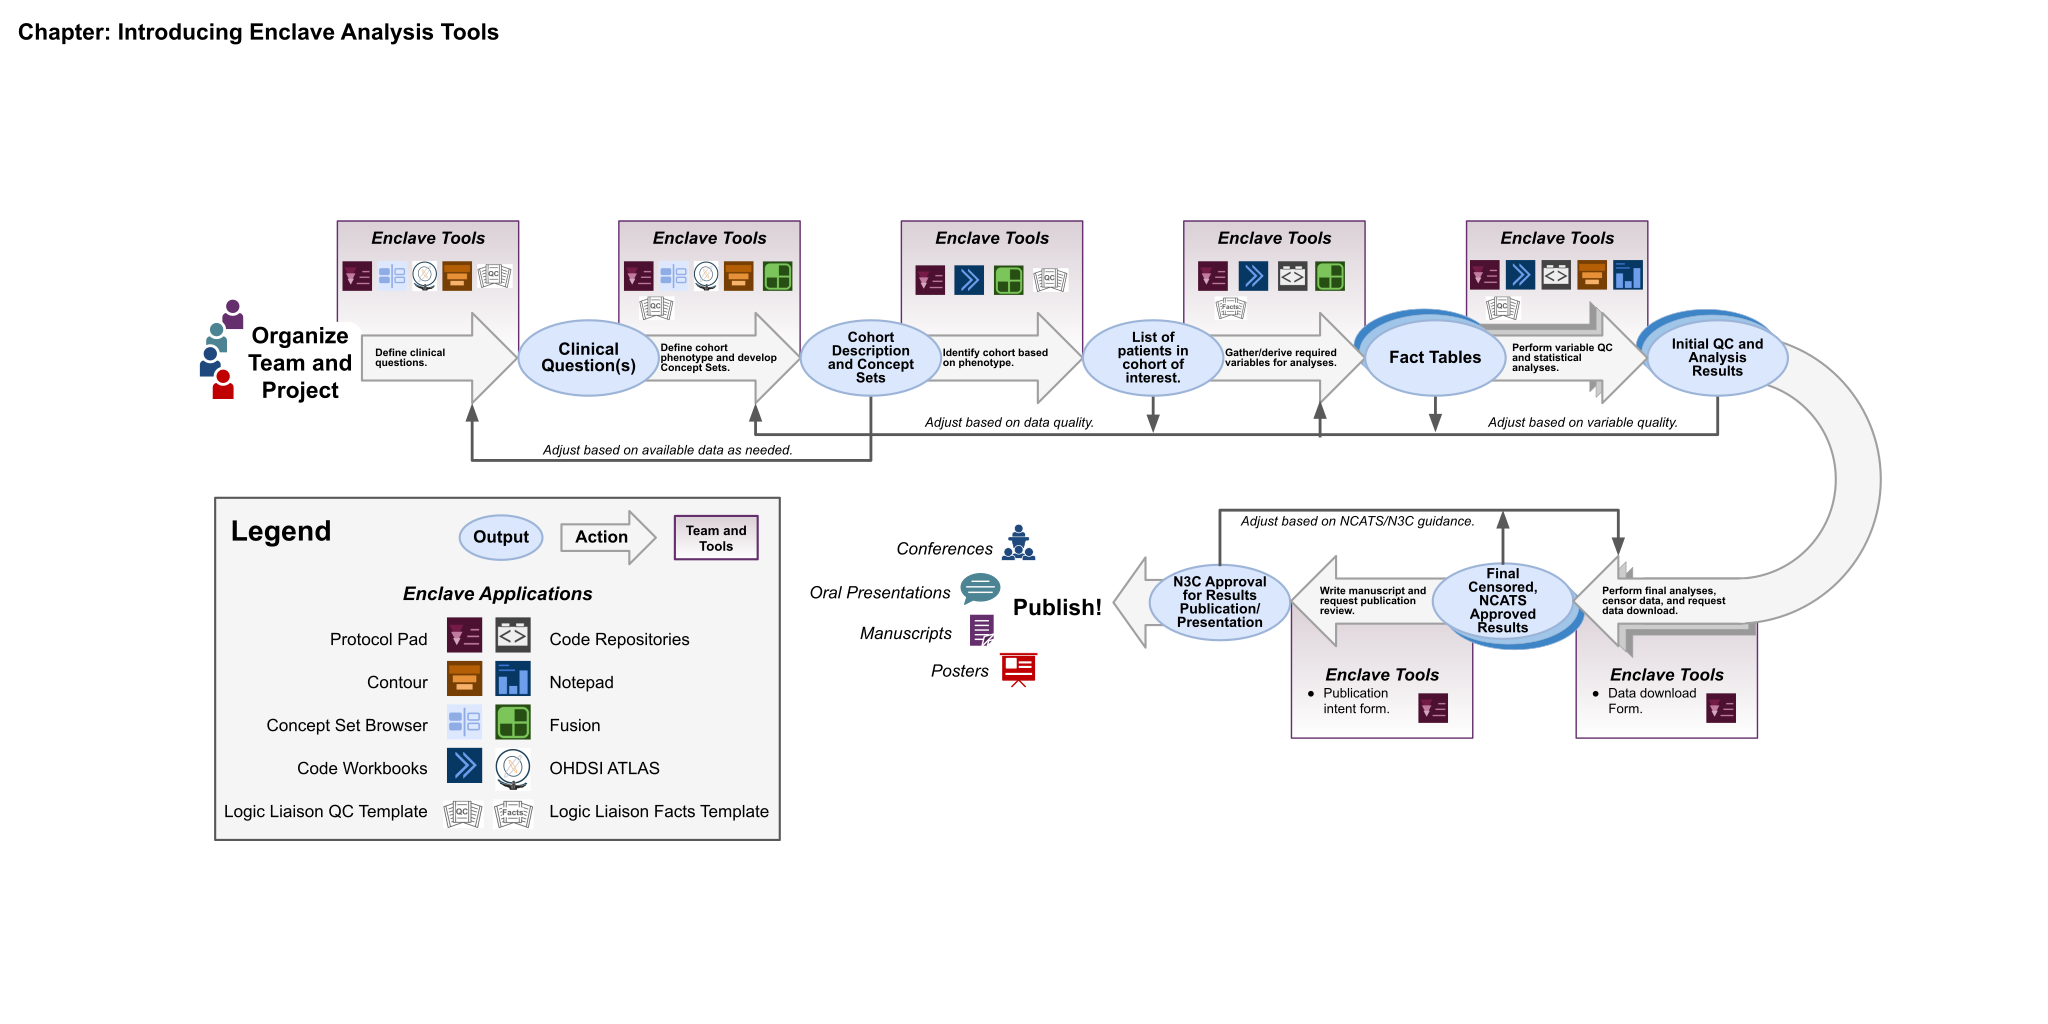
\includegraphics{chapters/images/enclave-tools/Fig1_ProjOverview_ToolsChapter.png}

}

\caption{alt\_text}

\end{figure}

Figure 1: High-level overview of an N3C project.

Due to the complexities of analyzing large clinical datasets, such as
that compiled in the N3C Enclave, it is common, and many times
necessary, to work in multidisciplinary collaborative teams to answer a
research question.
\protect\hyperlink{Figure1_IntroToTools_hiRes.png}{Figure 1} provides a
high-level overview of the process behind forming a team and performing
research using the N3C Enclave, along with the recommended field
expertise needed during each phase. It is important to note that while
certain team members may take the lead at various stages, a project
benefits if all team members are engaged to some degree at all phases.
Managing these collaborative and multi-faceted projects requires good
record keeping. The N3C Protocol Pad (see Section
\protect\hyperlink{N3C-Protocol-Pad}{X} in Chapter
\protect\hyperlink{Best-Practices-and-Important-Data-Considerations}{X})
is designed specifically for N3C research and to aid teams in designing,
implementing, reporting, and publishing their work in a Findable,
Accessible, Interoperable, and Reusable (FAIR) manner {[}1{]}{[}2{]}.
Thus it is recommended that you utilize this tool throughout the
implementation of your project.

A research project in N3C starts with organizing a team with the
required expertise (clinical, informatics, statistical, etc), followed
by defining clinical questions around COVID-19 and characterizing the
cohorts needed to answer each, i.e.~clinical phenotyping. Because the
N3C contains real-world EHR data that is harmonized from multiple data
models and dozens of institutions, some information needed to identify
an ideal clinical phenotype may be missing or incomplete. Thus, it is
important to assess what information is needed to create an N3C
computational phenotype for your cohorts. This could include using
conditions, labs, or medications as proxies to identify a cohort if some
information is not available. Generally, clinicians or other subject
matter experts are leading this process with informaticians/data
scientists providing guidance on what information is included in the N3C
Enclave, what is missing or sparse, and overall data quality (see
Chapter
\protect\hyperlink{Best-Practices-and-Important-Data-Considerations}{X}).
Some data quality aspects can be easily obtained through the use of
Logic Liaison Templates (see Section
\protect\hyperlink{Logic-Liaison-Fact-Tables-and-Templates}{X})
accessible through the N3C Knowledge Store. The N3C Enclave application
Contour (see Section \protect\hyperlink{Contour}{X}) can be utilized at
this stage, along with Code Workbooks (see Section
\protect\hyperlink{Code-Workbooks}{X}) for quick querying and
visualizing of the data. Additionally, Fusion (see Section
\protect\hyperlink{Fusion}{X}) can be utilized to keep track of
developed concept sets and utilized to easily input them into Logic
Liaison Templates.

The generation of a computational phenotype overlaps with the generation
of concept sets (see Section \protect\hyperlink{Concept-Sets}{X} in
Chapter \protect\hyperlink{Understanding-the-Data}{X} for details.), and
is often a cyclical process. Well-vetted concept sets are key to
obtaining robust cohorts, thus, having a team member familiar with the
organization of data and the OMOP vocabulary, such as a data liaison,
who can work closely with a clinician is beneficial. Concept set
generation can be done using the N3C Enclave Concept Set Browser, or
externally through OHDSI ATLAS.

Informaticians and data scientists then utilize the computational
phenotype and vetted concept sets to generate fact tables (i.e.~datasets
containing information about each patient like demographics,
comorbidities, lab results, etc) for the cohorts of interest using the
raw OMOP tables, which requires specific knowledge of how to work with
large datasets in a Spark environment. Fact tables include all the
information needed to characterize a cohort and perform downstream
analyses to answer your research questions. Facts can include patient
demographics, socioeconomic status, COVID status/severity, medications,
comorbidities, etc. Logic Liaison Fact Table Templates can provide you a
boost by allowing fast and robust generation of commonly used facts
using N3C vetted concept sets and peer-reviewed code as a starter table.
You can then append this base fact table to include project-specific
facts needed for analyses. Figures 6 and 7 in the N3C Knowledge Store
section of this chapter provide a more detailed view of how Logic
Liaison Templates can be integrated into a project to expedite fact
table generation. The generation of the original fact tables from raw
OMOP tables can be done using Code Workbooks (see Section
\protect\hyperlink{Code-Workbooks}{X}) or Code Repositories (see Section
\protect\hyperlink{Code-Repositories}{X}).

Data scientists and statisticians can then analyze the extracted and
formatted fact tables. This includes statistical tests, summary tables,
visualizations, and reports for the team to discuss. Data analysis is
also a cyclical process with all team members engaged in assessing
results and circling back to further refine the computational phenotype
and concept sets if needed. Depending on the type of analysis needed,
Code Workbooks (see Section \protect\hyperlink{Code-Workbooks}{X}) or
Contour (see Section \protect\hyperlink{Contour}{X}) can be utilized at
this step, followed by Foundry's Notepad (see Section
\protect\hyperlink{Notepad}{X}) for reporting out results for secure
team dissemination within the Enclave environment.

Once you obtain results that you wish to share with others, all tables,
figures, and other data needed for reporting in publications, conference
submissions, presentations, or any other activity outside the N3C
Enclave environment must be submitted as a Data Download Request for a
download review by NCATS (see Chapter
\protect\hyperlink{Publishing-and-Sharing-Your-Work}{X}). The download
request is meant to ensure no prohibited data is being downloaded as per
the \href{https://covid.cd2h.org/download}{N3C Data Download Policy}
summarized in the Publishing and Sharing Your Work chapter. After
approval, your results can be included in research outputs, such as
publications, and then submitted to the Publication Review Committee
(see Chapter \protect\hyperlink{Publishing-and-Sharing-Your-Work}{X}).
This step is necessary to ensure data are being reported properly in the
context of the research project and that proper attribution is being
given to all those who contributed to the success of the research,
either directly or indirectly. Upon approval, you are free to submit to
the venue of choice and freely present the approved data to anyone at
any time. Data download requests are performed within the Enclave
environment, followed by submitting a
\href{https://www.google.com/url?q=https://docs.google.com/forms/d/e/1FAIpQLSe8cezMX5KMXyo8DRb9qmgr95rAPEKcvIWIdZv72rIUxlcpIA/viewform\&sa=D\&source=docs\&ust=1677168810532504\&usg=AOvVaw12T-1ZD5cVj92DGadpr1IN}{Google
Form to the Publication Review Committee}.

The following sections of this chapter discuss each of the features and
applications needed to perform research in the N3C Enclave, and include
links to external Palantir documentation, as well as direct the reader
to other chapters of this book that contain a deeper dive into various
N3C topics, such as the organization of data and best practices. This
chapter is best utilized along side the information provided in the next
chapter, Best Practices and Important Data Considerations (see Chapter
\protect\hyperlink{Best-Practices-and-Important-Data-Considerations}{X}),
which includes information on recommended data workflows, such as
scheduling automatic data builds, to keep your research current,
managing your projects using the Protocol Pad, and much more.

\hypertarget{using-concept-sets}{%
\section{Using Concept Sets}\label{using-concept-sets}}

As discussed in the previous chapter Understanding the Data (see Chapter
\protect\hyperlink{Understanding-the-Data}{X}), the electronic health
information coded in the various vocabularies used across the country
are mapped to the OMOP common data model. By leveraging the hierarchical
structure, parent codes and descendants can be captured in one fell
swoop to create intensional concept sets for use in analysis.

{\textgreater\textgreater\textgreater\textgreater\textgreater{}
gd2md-html alert: inline image link here (to images/image2.png). Store
image on your image server and adjust path/filename/extension if
necessary. }(Back to top)(Next
alert){\textgreater\textgreater\textgreater\textgreater\textgreater{} }

\begin{figure}

{\centering \includegraphics{chapters/images/image2.png}

}

\caption{alt\_text}

\end{figure}

Figure 2: Concept Set Browser Homepage

The Concept Set Browser shown in {[}Figure
2{]}\#Figure2\_csetbrowser\_homepage.png is an N3C specific tool that
allows you to explore and modify existing concept sets as well as create
new concept sets to fit your exact study needs. For more details around
the process of concept set creation, read the Concept Sets section (see
Section \protect\hyperlink{Concept-Sets}{X} in Chapter
\protect\hyperlink{Understanding-the-Data}{X}). It is recommended that,
if you are a new researcher, you start your search for a concept set
with the list of N3C Recommended concept sets. These concept sets have
been frozen in their validated state by the
\href{https://covid.cd2h.org/liaisons}{Logic Liaisons and the Data
Liaisons} after obtaining clinician and informatic reviews (see Section
\protect\hyperlink{N3C-Recommended-concept-sets}{X} in Chapter
{[}X{]}\#Understanding-the-Data)). They are also the ones used to
identify common comorbidities and other facts on the Phenotype Explorer
and in the Logic Liaison Fact Table templates. The recommended other
method of finding commonly used concept sets is by exploring bundles
within the Concept Set Browser. These are groups of concept sets that
are often used together. Further exploration of all other concept sets
in the Concept Set Browser is also an option, though only advised when
proceeding with the understanding that many of the existing concept sets
that are not part of the N3C Recommended or bundles are crafted to be
specific to one particular study team's requirements.

Once concept sets have been identified for use in your analysis through
the Concept Set Browser, the concept set members table becomes the link
between concepts and the encompassing concept set as shown by {[}Figure
3{]}\#Figure3\_csetmembers\_table.png. You then have to ``point'' the
code to the concept set members table to access this linkage. Once this
has been accomplished, the choice becomes using the most recent version
of a concept set (concept\_set\_members.concept\_set\_name where
most\_recent\_version = TRUE) or using a specific version of the concept
set (concept\_set\_members.codeset\_id = \{codeset id value\}). While
there are alternative ways to utilize concept sets and concept ids, the
method described above is highly recommended primarily for the ability
to quickly update a concept set without having to find and change
hard-coded concept ids in a data processing pipeline.

{\textgreater\textgreater\textgreater\textgreater\textgreater{}
gd2md-html alert: inline image link here (to images/image3.png). Store
image on your image server and adjust path/filename/extension if
necessary. }(Back to top)(Next
alert){\textgreater\textgreater\textgreater\textgreater\textgreater{} }

\begin{figure}

{\centering \includegraphics{chapters/images/image3.png}

}

\caption{alt\_text}

\end{figure}

Figure 3: concept\_set\_members table

Referring to a concept set by name and using the most recent version is
often the preferred method for concept sets marked as N3C Recommended
since these concept sets can only be updated by N3C core contributors
after they have gone through a validation process which has been
described in the previous chapter Understanding the Data (see Chapter
\protect\hyperlink{Understanding-the-Data}{X}). For concept sets that
have not undergone the validation process and have not been marked as
N3C Recommended by the N3C core contributors, it is recommended that the
research team performs their own validation on an existing concept set
or creates a new concept set with the input of a clinician. The concept
set should then be referenced using its codeset ID when you are
performing your data analysis. This will allow your team to perform
their analysis from start to finish without worry about unvalidated
modifications to the concept set. However, the codeset id being
referenced in the code may need to be updated if the team chooses to
modify the concept set once starting the analysis. In constructing
phenotypes from concept sets, concept sets may also need to be joined
together; these actions are best done in SQL/R/Python code workbook (see
Section \protect\hyperlink{Code-Workbook}{X}) transforms with the use of
the
\href{https://unite.nih.gov/workspace/module/view/latest/ri.workshop.main.module.3ab34203-d7f3-482e-adbd-f4113bfd1a2b?id=KO-DE908D4\&view=focus}{Logic
Liaison's Combined Variable template} or in code repositories (see
Section \protect\hyperlink{Code-Repositories}{X}).

\hypertarget{n3c-knowledge-store}{%
\section{N3C Knowledge Store}\label{n3c-knowledge-store}}

The N3C Knowledge Store is an application where you, as an Enclave user,
can discover shared code templates, external datasets, reports, cohorts,
and Python libraries (collectively also known as Knowledge Objects or
KOs) and share similarly re-usable Knowledge Objects of your own with
other Enclave users, regardless of the specific project from which the
resource originated. Most Knowledge Store (KS) objects come about as
core contributors and researchers alike develop resources they believe
may be useful for others either within or outside of their research
project team and wish to share them with the broader community. If you
find yourself in this situation, you can easily create, submit, and
share a KS resource by following this
\href{https://unite.nih.gov/workspace/report/ri.report.main.report.1d9ad825-30d1-475c-b77b-88836af5ea2c}{Code
Workbook Template Quick Start Guide}. Otherwise, more specifics on how
to navigate the KS can be found in this
\href{https://unite.nih.gov/workspace/report/ri.report.main.report.7ac7904d-bbc3-4678-a224-8b8b7c12d40e}{Knowledge
Store Guide} within the Enclave.

\hypertarget{datasets}{%
\subsection{Datasets}\label{datasets}}

Of the many types of Knowledge Objects, the most common are datasets and
code templates. Datasets in the Knowledge Store can be internal or
external. Internal datasets are generated from data inside the enclave,
typically by researchers as part of their project, and are often of
patient or row level granularity. As described in the previous chapter
Understanding the Data, external datasets found in the Knowledge Store
provide a wealth of information from public datasets that have been
brought into the Enclave along with the crosswalks necessary for joining
these aggregate data to person level data at various levels of
granularity (see Section
\protect\hyperlink{Publicux2fExternal-Datasets}{X} in Chapter
\protect\hyperlink{Understanding-the-Data}{X}). Either type of dataset
can be imported into a workbook or code repository of the appropriate
data access level to be used as a starting point for further
transformation or analysis.

\hypertarget{code-templates}{%
\subsection{Code Templates}\label{code-templates}}

Depending on the author's intended use, some code templates can be
applied to your custom input dataset while other code templates produce
a dataset that can be joined to your study dataset. The code templates
themselves can also be imported and customized to produce a dataset for
defining a study cohort with key information to use during analysis or
simply used as example logic if you are newer to coding. Code templates,
in general, are often meant to help transform the massive amount of raw
data to smaller, more digestible, and more readily applicable datasets
and facts. A few helpful starter templates are those produced by the
\href{https://covid.cd2h.org/liaisons}{Logic Liaisons}, some of which
can be seen in {[}Figure 4{]}\#Figure4\_knowledgestore\_homepage.png.

{\textgreater\textgreater\textgreater\textgreater\textgreater{}
gd2md-html alert: inline image link here (to images/image4.png). Store
image on your image server and adjust path/filename/extension if
necessary. }(Back to top)(Next
alert){\textgreater\textgreater\textgreater\textgreater\textgreater{} }

\begin{figure}

{\centering \includegraphics{chapters/images/image4.png}

}

\caption{alt\_text}

\end{figure}

Figure 4: N3C Knowledge Store Homepage

\hypertarget{logic-liaison-fact-tables-and-templates}{%
\subsubsection{Logic Liaison Fact Tables and
Templates}\label{logic-liaison-fact-tables-and-templates}}

The Logic Liaison Fact Tables and Templates are specifically designed to
provide a validated and community agreed-upon method for calculating
particular facts at the date level and/or the patient level. Through
surveying the Domain Team Leads to establish a list of commonly derived
variables and continuous feedback from the N3C Community to refine and
update this list, the \href{https://covid.cd2h.org/liaisons}{Logic
Liaisons} have developed, disseminated, and maintain two main fact table
templates and an additional fact table template for SDoH variables.
These two main fact table templates each produce day-level and
person-level data frames of commonly used derived base variables for
\href{https://unite.nih.gov/workspace/module/view/latest/ri.workshop.main.module.3ab34203-d7f3-482e-adbd-f4113bfd1a2b?id=KO-BA3B835\&view=focus}{all
N3C patients} as well as a subset who have an index date for their acute
COVID-19 infection, the
\href{https://unite.nih.gov/workspace/module/view/latest/ri.workshop.main.module.3ab34203-d7f3-482e-adbd-f4113bfd1a2b?id=KO-BE5C652\&view=focus}{confirmed
COVID-19 positive patients} (PCR/AG positive or U07.1 COVID-19
diagnosed). These day-level and person-level datasets are commonly
referred to as the Logic Liaison Fact Tables and can be imported
directly into a workbook for use without modifying the template. These
fact tables are produced using a default set of concept sets from the
N3C Recommended Concept Sets list and a set of default values for the
template's parameters.

The main fact table template KOs include not only the shared logic for
importing/customizing the template for both data access levels, but also
a detailed README, example datasets (aka default Logic Liaison Fact
Tables), and example code workbooks as exemplified by {[}Figure
5{]}\#Figure5\_knowledgestore\_exampleKO.png. It is recommended you
first open the README and example code workbooks to see how the default
fact tables are generated and then decide whether you would like to use
the fact tables as they are or import the template to customize concept
sets and/or template parameter values to generate your project specific
version of the fact tables. The
\href{https://unite.nih.gov/workspace/module/view/latest/ri.workshop.main.module.3ab34203-d7f3-482e-adbd-f4113bfd1a2b?id=KO-1803D6D\&view=focus}{SDoH
Variables ALL PATIENTS} template provides you with a curated set of 70
geographically-based SDoH measures tied to each patient. Because joining
this data requires a valid five digit zip code, these fields are only
available for patients with a five digit zip code in Level 3 (LDS) data.

{\textgreater\textgreater\textgreater\textgreater\textgreater{}
gd2md-html alert: inline image link here (to images/image5.png). Store
image on your image server and adjust path/filename/extension if
necessary. }(Back to top)(Next
alert){\textgreater\textgreater\textgreater\textgreater\textgreater{} }

\begin{figure}

{\centering \includegraphics{chapters/images/image5.png}

}

\caption{alt\_text}

\end{figure}

Figure 5: Example Logic Liaison Fact Table Template Knowledge Object

The \href{https://covid.cd2h.org/liaisons}{Logic Liaisons} have also
developed, disseminated, and maintained a handful of overall data
quality templates, ancillary fact table, and ancillary data quality
templates in the Knowledge Store. {[}Figure
6{]}\#Figure6\_LLtemplate\_application.png depicts how one could apply
the set of Logic Liaison Templates to generate augmented fact tables
with a goal of asking one or more research questions within that
project.

{\textgreater\textgreater\textgreater\textgreater\textgreater{}
gd2md-html alert: inline image link here (to images/image6.png). Store
image on your image server and adjust path/filename/extension if
necessary. }(Back to top)(Next
alert){\textgreater\textgreater\textgreater\textgreater\textgreater{} }

\begin{figure}

{\centering \includegraphics{chapters/images/image6.png}

}

\caption{alt\_text}

\end{figure}

Figure 6: Example Application of Logic Liaison Overall Quality, Fact
Table, and Ancillary Fact Templates

The data quality templates provide a variety of data tables and
visualizations. The first two of which provide a method for evaluating
overall quality of the harmonized data ingested from sites.

\begin{itemize}
\tightlist
\item
  \href{https://unite.nih.gov/workspace/module/view/latest/ri.workshop.main.module.3ab34203-d7f3-482e-adbd-f4113bfd1a2b?id=KO-C3B0BBE\&view=focus}{Data
  Density by Site and Domain}

  \begin{itemize}
  \tightlist
  \item
    Calculates the Standardized Density, Median Absolute Deviation
    (MAD), and Directional Median Deviations (DMD) with respect to the
    number of unique patient/concept/days for each of the major OMOP
    tables (i.e.~condition\_occurrence, drug\_exposure, etc) and uses
    them to create a heatmap displaying how many MADs each site is from
    the median for each OMOP table. The template also scores the site's
    date shifting practices.
  \end{itemize}
\item
  \href{https://unite.nih.gov/workspace/module/view/latest/ri.workshop.main.module.3ab34203-d7f3-482e-adbd-f4113bfd1a2b?id=KO-D00A6DC\&view=focus}{Whitelist
  Filtering}

  \begin{itemize}
  \tightlist
  \item
    Creates a bar plot showing whitelisted data partners that have, at
    minimum, a certain percentage of COVID patients associated with a
    specified measurement, condition, drug, procedure, etc. Sites not
    meeting the minimum requirement are removed from the whitelist.
    These tables can be used in downstream filtering to keep only sites
    meeting the user-defined minimum data quality.
  \end{itemize}
\end{itemize}

Once the main fact table templates mentioned earlier this section have
been applied to generate the base fact tables, the ancillary fact
templates utilize the day-level and person-level datasets of the base
fact templates to efficiently generate additional derived variables
based on broadly requested and applicable logic such as:

\begin{itemize}
\tightlist
\item
  \href{https://unite.nih.gov/workspace/module/view/latest/ri.workshop.main.module.3ab34203-d7f3-482e-adbd-f4113bfd1a2b?id=KO-4BE516B\&view=focus}{Vaccine
  Fact}

  \begin{itemize}
  \tightlist
  \item
    Creates a vaccine fact table at the person level that summarizes
    their vaccination information
  \end{itemize}
\item
  \href{https://unite.nih.gov/workspace/module/view/latest/ri.workshop.main.module.3ab34203-d7f3-482e-adbd-f4113bfd1a2b?id=KO-23CE9BD\&view=focus}{Study
  Specific Fact Indexing}

  \begin{itemize}
  \tightlist
  \item
    Summarizes the indicators of a visit-level patient fact table with
    respect to whether they were present pre-, post-, or in a
    user-defined window surrounding an index date corresponding to a
    study-specific event. This template is similar to the All Patients
    Facts Tables with the exception that it is organized around a
    study-specific event rather than COVID diagnosis.
  \end{itemize}
\item
  \href{https://unite.nih.gov/workspace/module/view/latest/ri.workshop.main.module.3ab34203-d7f3-482e-adbd-f4113bfd1a2b?id=KO-DE908D4\&view=focus}{Combined
  Variables ALL PATIENTS}

  \begin{itemize}
  \tightlist
  \item
    Allows you to combine two variables (variable 1 and variable 2) in a
    visit-level table by creating a new ``same-day occurrence variable''
    indicating that both variables appear that day for that patient. You
    can also choose to make an ``either/or'' variable in the visit-level
    table that combines two variables (variable 3 and variable 4) into a
    new variable that flags days where at least one of the input
    variables is recorded for that patient.
  \end{itemize}
\item
  \href{https://unite.nih.gov/workspace/module/view/latest/ri.workshop.main.module.3ab34203-d7f3-482e-adbd-f4113bfd1a2b?id=KO-DA00725\&view=focus}{Combined
  Variables COVID PATIENTS}

  \begin{itemize}
  \tightlist
  \item
    Same as above except for patients with facts found based on their
    covid index date.
  \end{itemize}
\item
  \href{https://unite.nih.gov/workspace/module/view/latest/ri.workshop.main.module.3ab34203-d7f3-482e-adbd-f4113bfd1a2b?id=KO-06D5DA0\&view=focus}{CCI
  Score}

  \begin{itemize}
  \tightlist
  \item
    Provides an all-time score or a before-or-day-of-covid score
    (depending on your selection in the template) per patient based on
    the CCI weights {[}3{]}.
  \end{itemize}
\end{itemize}

{[}Figure 7{]}\#Figure7\_LLtemplate\_application2.png is a continuation
of Figure 3 to demonstrate how you could continue to apply the Logic
Liaison Templates to the augmented fact table created in order to answer
their specific research question within a project.

{\textgreater\textgreater\textgreater\textgreater\textgreater{}
gd2md-html alert: inline image link here (to images/image7.png). Store
image on your image server and adjust path/filename/extension if
necessary. }(Back to top)(Next
alert){\textgreater\textgreater\textgreater\textgreater\textgreater{} }

\begin{figure}

{\centering \includegraphics{chapters/images/image7.png}

}

\caption{alt\_text}

\end{figure}

Figure 7: Example Application of Logic Liaison Ancillary Quality
Templates

The ancillary data quality templates are intended to be applied to fact
tables after cohort creation and initial variable creation to stratify
question specific facts by site.

\begin{itemize}
\tightlist
\item
  \href{https://unite.nih.gov/workspace/module/view/latest/ri.workshop.main.module.3ab34203-d7f3-482e-adbd-f4113bfd1a2b?id=KO-E8BD195\&view=focus}{Systematic
  Missingness by Site and Study Variable}

  \begin{itemize}
  \tightlist
  \item
    Produces a final visualization that has a binary indicator for
    whether or not a site is systematically missing meaningful data for
    the study variables in the input dataset
  \end{itemize}
\item
  \href{https://unite.nih.gov/workspace/module/view/latest/ri.workshop.main.module.3ab34203-d7f3-482e-adbd-f4113bfd1a2b?id=KO-9901C7E\&view=focus}{Fact
  Density by Site Visualization}

  \begin{itemize}
  \tightlist
  \item
    Calculates the Standardized Density, Median Absolute Deviation
    (MAD), and Directional Median Deviations (DMD) with respect to the
    numerical values in each column of the input table (any
    non-numerical field is converted to a binary value using the
    isNotNull() function) and creates heatmaps to visualize the metrics.
  \end{itemize}
\end{itemize}

Once you obtain results you wish to share outside of the Enclave for a
project, the results must undergo a Data Download Request before being
available to export outside of the Enclave. Additional details around
exporting results can be found in the Publishing and Sharing Your Work
chapter (see Chapter
\protect\hyperlink{Publishing-and-Sharing-Your-Work}{X}). Training
materials for getting started with Logic Liaison Templates are available
\href{https://unite.nih.gov/workspace/module/view/latest/ri.workshop.main.module.e7b83a8c-545e-49ac-8714-f34bfa7f7767?view=focus\&Id=26}{here}
within the Enclave. Outside of the main confirmed COVID+ template and a
subset of columns in All Patients, these templates could be generalized
to apply to research projects outside of the Enclave where studies do
not necessarily need to fall within the scope of COVID-19.

While it is not necessary to utilize Knowledge Store resources when
conducting your research project, it does allow you to get a jumpstart
on gathering and understanding the data by avoiding effort duplication
and providing a general starting point. You can then build upon this
fact table using the ancillary templates that allow self-definition of
the index event, combining variables, generating a CCI score, and
associating SDoH variables based on zip code crosswalks. The Logic
Liaison ancillary data quality templates provide the same structure for
analyzing data missingness, density, and contribution quality by site.
Further explanation as to why these Knowledge Store objects are highly
applicable can be found in the Best Practices and Important Data
Considerations chapter (see Chapter
\protect\hyperlink{Best-Practices-and-Important-Data-Considerations}{X}).

\hypertarget{n3c-enclave-applications}{%
\section{N3C Enclave Applications}\label{n3c-enclave-applications}}

This section will cover the usage of various applications made available
in the N3C Enclave, including Protocol Pad, Contour, Code Workbooks, and
more
(\href{https://www.palantir.com/docs/foundry/getting-started/application-reference/}{a
complete list of Foundry applications can be found here}). Before
designing and running an analysis utilizing data in the Enclave, it
helps to understand the concepts of a
``\href{https://www.palantir.com/docs/foundry/data-integration/data-pipeline/}{data
pipeline}'' and a
``\href{https://www.palantir.com/docs/foundry/pipeline-builder/core-concepts/}{data
transform}'' as well as how the data are stored and accessed via Apache
Spark on a distributed file system. For those unfamiliar with these
concepts a high-level overview, along with links to documentation on
code optimization in the N3C Enclave, can be found in Section {[}X{]} of
Chapter \protect\hyperlink{ux3fux3fux3f}{X}.

\hypertarget{n3c-protocol-pad}{%
\subsection{N3C Protocol Pad}\label{n3c-protocol-pad}}

N3C Documentation:
\href{https://unite.nih.gov/workspace/notepad/view/ri.notepad.main.notepad.8e97750f-d764-4df9-bb25-42ab32fcaa26}{Quick
Start Guide} and
\href{https://unite.nih.gov/workspace/notepad/view/ri.notepad.main.notepad.9d509aa3-7c76-42b3-a891-076a6f450f37}{Detailed
Instructions}

\begin{itemize}
\tightlist
\item
  Electronic lab notebook
\item
  Promote collaboration, organize work, and translation to final
  manuscript
\item
  Methodology checklist
\end{itemize}

{\textgreater\textgreater\textgreater\textgreater\textgreater{}
gd2md-html alert: inline image link here (to images/image8.png). Store
image on your image server and adjust path/filename/extension if
necessary. }(Back to top)(Next
alert){\textgreater\textgreater\textgreater\textgreater\textgreater{} }

\begin{figure}

{\centering \includegraphics{chapters/images/image8.png}

}

\caption{alt\_text}

\end{figure}

Figure 8: N3C Protocol Pad Homepage

Before diving into an analysis, it is highly recommended that you use
N3C's Protocol Pad shown in {[}Figure
8{]}\#Figure8\_protocolpad\_homepage.png to organize your thoughts and
path forward. Research studies can span many months and pass through the
hands of many team members before reaching a stage where you may want to
share the results through publication or other approved means. The
Protocol Pad serves as an electronic lab notebook to help organize
tasks, track progress, and document results in a cohesive format
throughout the process of reaching a study's final state. As a result of
this organization and tracking, the tool facilitates easy translation of
the work, decisions, and contributors to producing a final manuscript if
that is the goal of the protocol.

Protocol Pad is the foundation for performing reproducible and
repeatable science within the N3C Enclave. The templates, checklists,
and links to key resources provided within the tool guide you along the
path of well structured division of labor and use of best practices when
performing research using the observational data in the Enclave. The
tool also assists your team in keeping the work in alignment with the
project. A more in depth explanation of how Protocol Pad can facilitate
research can be found in the Best Practices and Important Data
Considerations chapter (see Chapter
\protect\hyperlink{Bestux5cux2520Practices-and-Important-Data-Considerations}{X}).
Documentation on the tool's functionality can be found in this
\href{https://unite.nih.gov/workspace/notepad/view/ri.notepad.main.notepad.8e97750f-d764-4df9-bb25-42ab32fcaa26}{Quick
Guide} as well as this more
\href{https://unite.nih.gov/workspace/notepad/view/ri.notepad.main.notepad.9d509aa3-7c76-42b3-a891-076a6f450f37}{Detailed
Guide}.

\hypertarget{contour}{%
\subsection{Contour}\label{contour}}

Palantir Documentation:
\href{https://www.palantir.com/docs/foundry/contour/overview/}{Contour
Overview}

\begin{itemize}
\tightlist
\item
  Programming-free analysis interface
\item
  Point-and-Click data analysis pipeline development
\item
  Data summary and visualization
\item
  Allows customization with Contour's expression language
\item
  Dashboard development
\end{itemize}

{\textgreater\textgreater\textgreater\textgreater\textgreater{}
gd2md-html alert: inline image link here (to images/image9.png). Store
image on your image server and adjust path/filename/extension if
necessary. }(Back to top)(Next
alert){\textgreater\textgreater\textgreater\textgreater\textgreater{} }

\begin{figure}

{\centering \includegraphics{chapters/images/image9.png}

}

\caption{alt\_text}

\end{figure}

Figure 9: Example Contour Analysis

The Contour application is a programming-free interface to the N3C
Enclave that allows those with limited knowledge of Python, R, and SQL
to create top-down analysis pipelines in a point-and-click fashion, as
well as generate dynamically updated dashboards. A Contour analysis
starts by specifying the path to the input dataset as shown in {[}Figure
9{]}\#Figure9\_contour\_example.png. Subsequent transforms of that
dataset are then specified, which can include adding/calculating new
columns, filtering rows or columns, joining with other datasets,
creating summary figures and charts, summarizing tables through
pivoting, and more. Contour's
\href{https://www.palantir.com/docs/foundry/contour/expressions-overview/}{expression
language} also allows for more complex querying and data aggregation
beyond the default operations provided. Once an analysis is complete,
resulting datasets can be saved to the Enclave for use in additional
Contour pipelines or other Enclave applications, like Code Workbooks
(see Section \protect\hyperlink{Code-Workbooks}{X}. Contour can also
quickly create summary figures from source tables without code, and has
a variety of visualization options, including bar charts, histograms and
heatmaps.

Figures or summary tables created in Contour can be exported to a
dashboard within Contour. Contour Dashboards allows chart-to-chart
filtering, and an easy drag-and-drop interface to build the dashboard
while iterating on an analysis. A dashboard is dynamic and interactive,
allowing the reader to adjust the graphs to better explore analysis
results in a guided and structured way. Figures generated in a Contour
analysis can also be exported to other Enclave applications like Notepad
for reporting out results. The main difference between Notepad (see
Section \protect\hyperlink{Notepad}{X}) and a Contour Dashboard is that
Notepad provides a static report with figures that cannot be dynamically
changed by the reader. A detailed orientation to Contour can be found in
the Foundry Documentation
\href{https://www.palantir.com/docs/foundry/contour/overview/}{here}.

\hypertarget{code-workbooks}{%
\subsection{Code Workbooks}\label{code-workbooks}}

Tutorial:
\href{https://unite.nih.gov/workspace/module/view/latest/ri.workshop.main.module.e7b83a8c-545e-49ac-8714-f34bfa7f7767?view=focus\&Id=22}{Intro
to Code Workbook}

Palantir Documentation:
\href{https://www.palantir.com/docs/foundry/code-workbook/overview/}{Code
Workbook Overview}

\begin{itemize}
\tightlist
\item
  Graphical organization of logic
\item
  Simplification of code
\item
  Easy reuse of pre-authored logic
\item
  Add visualizations to reports
\item
  Supports Python, R, SQL, PySpark, and SparkR
\item
  Console debugging and development
\item
  Branching facilitates collaboration and reproducibility
\item
  Workspace to reuse templatized logic
\item
  Exporting code to GitHub
\end{itemize}

Code Workbook is a GUI-based application for you to apply code-based
transformations to datasets for the purpose of creating new datasets and
visualizations. The explicit goals of the application are to facilitate
a collaborative environment in which you can quickly iterate over logic
to produce artifacts interoperable with the suite of Enclave
applications. The default Code Workbook interface is structured as a
directed graph in which nodes represent either datasets or
transformations that output datasets. Edges represent the flow of data
through the graph such that upstream datasets are inputs for logical
operations performed by downstream code transforms. {[}Figure
10{]}\#Figure10\_EnclaveApplications.png shows an abstract version of a
Code Workbook, while {[}Figure
11{]}\#Figure11\_codeworkbook\_example.png is an actual screenshot in
the Enclave where data flows from the left to the right. Any dataset
which you have access to within the workspace where the Code Workbook is
located can be imported as an input to the various types of
transformations. For each transformation \emph{{one or more tables are
specified as the input}} and are transformed into a single output table
(Figure 10A). Multiple transformations can also be strung together
(Figure 10B) to create an analysis pipeline (see Palantir's
\href{https://www.palantir.com/docs/foundry/building-pipelines/overview/}{Anatomy
of a Data Pipeline} module for more detailed information, as well as
Chapter
\protect\hyperlink{Best-Practices-and-Important-Data-Considerations}{X}).
In Code Workbook, \emph{{the primary and required output of a
transformation is always a single table}}; however, visualizations such
as graphs and charts can also be generated and saved along the way. Note
that the code performing the transformation and the resulting output
table are always represented as a single node in the Code Workbook
interface.

{\textgreater\textgreater\textgreater\textgreater\textgreater{}
gd2md-html alert: inline image link here (to images/image10.png). Store
image on your image server and adjust path/filename/extension if
necessary. }(Back to top)(Next
alert){\textgreater\textgreater\textgreater\textgreater\textgreater{} }

\begin{figure}

{\centering \includegraphics{chapters/images/image10.png}

}

\caption{alt\_text}

\end{figure}

Figure 10: Abstracted view of data transforms

{\textgreater\textgreater\textgreater\textgreater\textgreater{}
gd2md-html alert: inline image link here (to images/image11.png). Store
image on your image server and adjust path/filename/extension if
necessary. }(Back to top)(Next
alert){\textgreater\textgreater\textgreater\textgreater\textgreater{} }

\begin{figure}

{\centering \includegraphics{chapters/images/image11.png}

}

\caption{alt\_text}

\end{figure}

Figure 11: Example Data Transformation Pipeline in Code Workbook

\hypertarget{types-of-transforms}{%
\subsubsection{Types of Transforms}\label{types-of-transforms}}

\begin{itemize}
\tightlist
\item
  \textbf{Manual Entry} transforms allow you to manually populate a
  custom dataset directly in the specific Code Workbook you are
  currently working in as a ``quick and dirty'' alternative to manually
  populating importable or referenceable datasets with Fusion (see
  Section \protect\hyperlink{Fusion}{X}).
\item
  \textbf{Python/PySpark Code} transforms contain a Python function that
  takes one or more datasets as input parameters and returns a single
  dataset as output.
\item
  \textbf{R/SparkR Code} transforms contain an R function that takes one
  or more datasets as input parameters, and outputs a single data frame.
\item
  \textbf{SQL Code} transforms let you write a Spark SQL query to create
  a new dataset from the available input datasets.
\item
  \textbf{Template }transforms are parameterized blocks of reusable code
  which you can configure from a point-and-click interface. Many code
  templates are available in the Knowledge Store (see
  Section\protect\hyperlink{N3C-Knowledge-Store}{X}), but you can create
  your own templates scoped to their workspace. Multiple single-node
  templates can be combined to create a multi-node template to allow
  reuse of entire configurable pipelines.
\item
  \textbf{Visualize }transforms offer a point-and-click interface for
  you to create figures and pivot tables. Note this transform is only
  available for use on saved datasets; it cannot accept unsaved
  transformations as an input parameter.
\end{itemize}

Both Python and R transforms can optionally return a single dataset and
produce visualizations using Python libraries/R packages. Any
visualization produced in a Code Workbook can subsequently be embedded
in a Notepad document. Datasets returned by a transform are ephemeral by
default, that is, the transform must be recomputed each time the dataset
is used as a downstream input, but options exist to conserve compute
power by either caching or saving the output. Caching stores the output
temporarily, while saving the dataset stores it permanently in the
Enclave. It is recommended that transforms in a pipeline requiring
significant compute be saved as datasets to reduce iteration time during
development. In addition to manually clicking ``Run'' on a transform, a
\href{https://www.palantir.com/docs/foundry/building-pipelines/scheduling-overview/}{build
schedule} can be defined to recompute it at regular intervals based on a
trigger. You can choose the trigger to be the successful update of an
input dataset or simply the elapsing of a specified period of time. This
capability can best be visualized using the Data Lineage tool described
later in this chapter (see Section \protect\hyperlink{Data-Lineage}{X}).

The Console, Global Code, and Logs panels facilitate quick iteration and
code development and debugging. The
\href{https://www.palantir.com/docs/foundry/code-workbook/workbooks-console/}{Console}
allows you to interactively execute and check syntax in Python, R, or
SQL outside of a transform node.
\href{https://www.palantir.com/docs/foundry/code-workbook/workbooks-global-code/}{Global
Code} allows you to define custom functions available to all transforms
in the Code Workbook. Each code transform includes a Logs panel to view
console output generated by code and to view detailed stack traces when
transforms fail due to an error.

Many Python and R transforms rely on external libraries and packages
which can be made available via the
\href{https://www.palantir.com/docs/foundry/code-workbook/environment-overview/}{Environment
Configuration}. The Enclave provides default configurations tailored to
common use cases. For instance, the \emph{default} profile includes
common packages like pandas and tidyverse for routine analysis, whereas
the \emph{profile-high-memory} profile includes packages like
\href{https://www.palantir.com/docs/foundry/develop-models/python-models/}{foundry\_ml}
for machine learning. You can create your own Environment Configurations
which include packages meeting your project's specific needs.

Not all libraries and packages are included in the list of options, but
you can submit a ticket within the Enclave by clicking on \emph{Help \&
Support \textgreater{} Help Center \textgreater{} Report an Issue} to
request additional packages be made available. The Enclave maintains
instances of the default configurations on warm standby, allowing them
to be quickly initialized when you request a new environment. Custom
configurations require more time for initialization as instances of
these must be started from scratch rather than merely assigned. For this
reason, it is recommended to use default configurations when possible.

Following best practices for collaborative software development, Code
Workbook allows for
\href{https://www.palantir.com/docs/foundry/code-workbook/branching-overview/}{branching}
of the logic within a workbook. As with other popular version control
technologies (i.e.~\href{https://git-scm.com/}{Git}), branching allows
you to make copies of a workbook which your team members can develop
independently of the source workbook. Once the development in a
particular branch is deemed complete, it can be merged back into the
originating branch. Prior to the merge, you can preview both line-level
differences within each node, as well as node-level differences of nodes
that have been added/removed. Good practice dictates that you perform
all development on individual branches, which are then merged back into
a common \emph{master} branch.

Because the \emph{master} branch can change in the interval between you
creating a branch and merging it back in, it is important to preview
merge changes to ensure that the branch's contributions are both correct
and compatible with the current state of the \emph{master} branch.
However, note that your branch will be automatically deleted after it is
merged, which is an important difference from the normal Git behavior.
Another prime use case for code branching is to ensure the
reproducibility of a given dataset used in a research project. Because
the OMOP and N3C-curated datasets are also versioned, you can create a
code branch in which all input datasets are set to the same version
release (as shown in {[}Figure
12{]}\#Figure12\_codeworkbook\_pinningrelease.png) to effectively freeze
a dataset used in a specific analysis for later reproducibility while
still allowing the possibility of adding additional features.
User-generated datasets are set to the same branch as the Code Workbook
in which they were created. Finally, Code Workbooks allow you to collect
and download all coded transformations within a single workbook into a
Git repository that can be easily uploaded to GitHub for public
dissemination.

{\textgreater\textgreater\textgreater\textgreater\textgreater{}
gd2md-html alert: inline image link here (to images/image12.png). Store
image on your image server and adjust path/filename/extension if
necessary. }(Back to top)(Next
alert){\textgreater\textgreater\textgreater\textgreater\textgreater{} }

\begin{figure}

{\centering \includegraphics{chapters/images/image12.png}

}

\caption{alt\_text}

\end{figure}

Figure 12: Pinning to an input dataset's release version

Palantir has created extensive
\href{https://www.palantir.com/docs/foundry/code-workbook/overview/}{documentation}
of the Code Workbook application including tutorials. N3C has also
published
\href{https://unite.nih.gov/workspace/module/view/latest/ri.workshop.main.module.e7b83a8c-545e-49ac-8714-f34bfa7f7767?view=focus\&Id=22}{training
materials}.

\hypertarget{code-repositories}{%
\subsection{Code Repositories}\label{code-repositories}}

Palantir Documentation:
\href{https://www.palantir.com/docs/foundry/code-repositories/overview/}{Code
Repository Overview}

\begin{itemize}
\tightlist
\item
  Production pipelines
\item
  Code reuse across projects
\item
  Built in version control
\end{itemize}

{\textgreater\textgreater\textgreater\textgreater\textgreater{}
gd2md-html alert: inline image link here (to images/image13.png). Store
image on your image server and adjust path/filename/extension if
necessary. }(Back to top)(Next
alert){\textgreater\textgreater\textgreater\textgreater\textgreater{} }

\begin{figure}

{\centering \includegraphics{chapters/images/image13.png}

}

\caption{alt\_text}

\end{figure}

Figure 13: Example Code Repository

Code Repositories shown in {[}Figure
13{]}\#Figure13\_coderepo\_example.png are available within the N3C
enclave and should be used when you wish to share code across multiple
Code Workbooks or projects, or need to develop a robust production
pipeline. Code Repositories \emph{{do not support}} data visualization,
coding in R, or point-and-click templates. Additional
\href{https://www.palantir.com/docs/foundry/code-workbook/code-repositories-comparison/}{differences
between Code Repositories and Code Workbooks} can be found in the
Palantir Documentation. Palantir has also compiled several
\href{https://unite.nih.gov/workspace/documentation/product/foundry-training-portal/de_code-repo-environment_module1}{tutorials
on how to create, publish, and maintain Code Repositories.}

For any large analytic project, there are many pieces of code and other
artifacts that should be shared between different components within the
project. Some code is useful enough that it should be shared across
projects. Code Repositories provide a standard mechanism for
encapsulating reusable components and allowing them to be reused within
projects.

Underlying the Code Repository is the Git version control system. You
can edit and maintain code using all of the capabilities of Git
including comparing versions, branching and pull requests. Versions that
are tagged in Git will be automatically published in the Enclave as a
shared library, which allows you and others that have access to your
project space to import that code into other Code Workbooks (note this
requires you to create a customized environment that imports your code
specifically, which may increase workbook initialization time). If you
want to make your repository public so others outside of your project
workspace can use it you can do one of the following:

\begin{itemize}
\tightlist
\item
  Package your code into a properly structured python package. This
  allows other researchers from different project spaces to run it from
  their Code Workbooks or Repositories.
\item
  Submit the Code Repository to the Knowledge Store where it will then
  be visible to anyone who has Enclave access.
\item
  Publish the Code Repository to a public Github where the code will
  then become accessible to anyone outside the Enclave.
\end{itemize}

More information on Code Repositories can be found in the
\href{https://www.palantir.com/docs/foundry/code-repositories/overview/}{Palantir
Documentation}.

\hypertarget{fusion}{%
\subsection{Fusion}\label{fusion}}

Palantir Documentation:
\href{https://www.palantir.com/docs/foundry/fusion/overview/}{Fusion
Sheet Overview}

\begin{itemize}
\tightlist
\item
  Useful for writing back datasets for use within the Enclave
\item
  Leverage cell references and spreadsheet functions
\item
  Sync tables to a dataset to use in other Foundry applications
\item
  Create charts
\item
  Allow customization and flexibility
\end{itemize}

{\textgreater\textgreater\textgreater\textgreater\textgreater{}
gd2md-html alert: inline image link here (to images/image14.png). Store
image on your image server and adjust path/filename/extension if
necessary. }(Back to top)(Next
alert){\textgreater\textgreater\textgreater\textgreater\textgreater{} }

\begin{figure}

{\centering \includegraphics{chapters/images/image14.png}

}

\caption{alt\_text}

\end{figure}

Figure 14: Example Fusion Sheet

Fusion, shown in {[}Figure 14{]}\#Figure14\_fusion\_example.png, is a
spreadsheet application within the Enclave analogous to Microsoft Excel
or Google Sheets. Palantir provides
\href{https://www.palantir.com/docs/foundry/fusion/overview/}{extensive
documentation}. Fusion allows you to
\href{https://www.palantir.com/docs/foundry/fusion/sync-table-dataset/}{sync
specific cell ranges within a spreadsheet to Spark datasets}, which can
subsequently be imported into any other Enclave application. Fusion is
an excellent option for use cases which require manual data entry, such
as curating lists of concept sets (see Chapter
\protect\hyperlink{Understanding-the-Data}{X}) to configure the Logic
Liaison Fact Tables and Templates (see Section
\protect\hyperlink{N3C-Knowledge-Store}{X}). Unlike many other Enclave
applications, Fusion is not suitable for large datasets; each document
has a maximum size of 50 MB. Similar to Google Sheets, multiple users
can simultaneously view and edit the same document.

Fusion provides many features familiar to other spreadsheet applications
such as cell-referencing formulas, formatting, and a charting library to
name a few. While you cannot directly import external .xls/.xlsx
formatted files into the Enclave, you can copy/paste external dataset
values into Fusion. For example, you can copy and paste concept IDs from
\href{https://ohdsi.github.io/TheBookOfOhdsi/OhdsiAnalyticsTools.html\#atlas}{ATLAS}
to use in an analysis or metadata manually curated for a dataset. To
import larger external datasets into the N3C Enclave see Chapter
\protect\hyperlink{Chapterux5cux2520onux5cux2520externalux5cux2520datasets}{X},
and \href{https://zenodo.org/record/4574608\#.Y6IeG-zMJTZ}{N3C
procedures and protocols around importing large external datasets}. In
addition to standard spreadsheet functionality, Fusion has additional
features which allow it to integrate with the rest of your Enclave
environment. Objects created within Fusion, such as formatted tables,
can be embedded in Notepad (see Section \protect\hyperlink{Notepad}{X}).
Finally, Fusion sheets can be templatized to facilitate replication of
similar functionality.

\hypertarget{notepad}{%
\subsection{Notepad}\label{notepad}}

Palantir Documentation:
\href{https://www.palantir.com/docs/foundry/notepad/overview/}{Notepad
Overview}

\begin{itemize}
\tightlist
\item
  Note taking with ability to add embeds of the workflow
\item
  Documentation of pipelines or datasets
\item
  Create report templates
\item
  Monthly status reports using template function
\item
  Unable to create dashboard or complex page-based text editing
\end{itemize}

{\textgreater\textgreater\textgreater\textgreater\textgreater{}
gd2md-html alert: inline image link here (to images/image15.png). Store
image on your image server and adjust path/filename/extension if
necessary. }(Back to top)(Next
alert){\textgreater\textgreater\textgreater\textgreater\textgreater{} }

\begin{figure}

{\centering \includegraphics{chapters/images/image15.png}

}

\caption{alt\_text}

\end{figure}

Figure 15: Example Notepad Document

Many research projects in the Enclave are complex, involving multiple
summary datasets, statistical analyses, and visualizations scattered
across multiple applications and documents. Notepad is a tool that is
often used for consolidating various research artifacts from multiple
sources within the Enclave into a single coherent document as shown in
{[}Figure 15{]}\#Figure15\_notepad\_example.png. Formatted Fusion
tables, Contour charts, Python/R-generated images from Code Workbooks,
and more are all embeddable in a Notepad document, with the option to
add a title and caption for each artifact. Users can also create
sections and provide narrative structure to their documents using
\href{https://www.markdownguide.org/}{Markdown}. A Notepad document can
be arranged and configured using a point-and-click interface.

All embedded objects can be configured to remain static or refresh
automatically when the underlying data sources update. Notepad is also
useful for annotating documents, presenting an executive summary of
results for internal stakeholders, or external presentations after being
approved for download request and export as PDF. Logic Liaison Templates
(see Section
\protect\hyperlink{Logic-Liaison-Fact-Tables-and-Templates}{X}) in the
Knowledge Store generally includes a README which is created using
Notepad. The tool does have limitations in that it cannot be used to
create dashboards that include chart-to-chart filtering; however,
\href{https://www.palantir.com/docs/foundry/contour/dashboards-overview/}{Contour
Dashboards} can provide this feature for tabular data and
\href{https://www.palantir.com/docs/foundry/quiver/dashboards-overview/}{Quiver
Dashboards} can provide this feature for object or time series data.
Palantir has curated documentation for creating and editing
\href{https://www.palantir.com/docs/foundry/notepad/overview/}{Notepad}
documents. Palantir also has documentation for their application known
as
\href{https://www.palantir.com/docs/foundry/reports/overview/}{Reports}
that was previously used in a similar fashion though with less
functionality compared to Notepad.

\hypertarget{data-lineage-aka-monocle}{%
\subsection{Data Lineage (aka Monocle)}\label{data-lineage-aka-monocle}}

Palantir Documentation:
\href{https://www.palantir.com/docs/foundry/data-lineage/overview/}{Data
Lineage Overview}

\begin{itemize}
\tightlist
\item
  Find datasets
\item
  Expand or hide a dataset's ancestors and descendants
\item
  Visualize a data pipeline and its details
\item
  Facilitate dataset build scheduling
\end{itemize}

{\textgreater\textgreater\textgreater\textgreater\textgreater{}
gd2md-html alert: inline image link here (to images/image16.gif). Store
image on your image server and adjust path/filename/extension if
necessary. }(Back to top)(Next
alert){\textgreater\textgreater\textgreater\textgreater\textgreater{} }

\begin{figure}

{\centering \includegraphics{chapters/images/image16.gif}

}

\caption{alt\_text}

\end{figure}

Figure 16: Example Data Lineage Visualization

Whether you're creating a data pipeline for your research project or
investigating one from the Knowledge Store, you'll likely want to
holistically assess the dataset's origins with the Data Lineage tool
shown in {[}Figure 16{]}\#Figure16\_datalineage\_example.gif. The data
pipeline flows from left to right, which is an intuitive way to
visualize the relationships between datasets and their ancestors or
descendants. Views are enhanced with color-coding and grouping. The Data
Lineage tool allows you to view details such as a dataset's schema, last
build datetime, and the code that generated the dataset. You can use
this lineage tracing tool to understand and verify the data curation
methods when using Knowledge Objects and other shared datasets as part
of their study analysis. The Data Lineage tool also allows you to see
upstream dataset(s) aka potential triggers and downstream dataset(s) aka
potential targets for setting up dataset build schedules. Palantir
Documentation provides
\href{https://www.palantir.com/docs/foundry/data-lineage/overview/}{additional
instructions and descriptions} of Data Lineage.

References

{[}1{]} Wilkinson, M., Dumontier, M., Aalbersberg, I. et al.~The FAIR
Guiding Principles for scientific data management and stewardship.\_ Sci
Data\_ \textbf{3}, 160018 (2016).
\url{https://doi.org/10.1038/sdata.2016.18}

{[}2{]} \url{https://www.go-fair.org/fair-principles/}

{[}3{]} Charlson ME, Pompei P, Ales KL, MacKenzie CR. A new method of
classifying prognostic comorbidity in longitudinal studies: development
and validation. J Chronic Dis. 1987;40(5):373-83. doi:
10.1016/0021-9681(87)90171-8. PMID: 3558716.

\hypertarget{sec-practices}{%
\chapter{Best Practices and Important Data
Considerations}\label{sec-practices}}

\begin{tcolorbox}[enhanced jigsaw, rightrule=.15mm, colback=white, leftrule=.75mm, breakable, left=2mm, bottomtitle=1mm, opacityback=0, toprule=.15mm, colframe=quarto-callout-note-color-frame, titlerule=0mm, toptitle=1mm, coltitle=black, title=\textcolor{quarto-callout-note-color}{\faInfo}\hspace{0.5em}{Note}, bottomrule=.15mm, arc=.35mm, opacitybacktitle=0.6, colbacktitle=quarto-callout-note-color!10!white]

This chapter is being drafted in Google Docs at
\url{https://drive.google.com/drive/u/0/folders/1ExkYChsnO3hYZk6HCI5cEfQdQJ9F-ynw}

See a draft of the chapter outline at
\url{https://docs.google.com/document/d/1ttUKgwVcIZHM87elrlUNV6Qi9thzOwKBg8GegKObEtg/}

\end{tcolorbox}

\begin{tcolorbox}[enhanced jigsaw, rightrule=.15mm, colback=white, leftrule=.75mm, breakable, left=2mm, bottomtitle=1mm, opacityback=0, toprule=.15mm, colframe=quarto-callout-warning-color-frame, titlerule=0mm, toptitle=1mm, coltitle=black, title=\textcolor{quarto-callout-warning-color}{\faExclamationTriangle}\hspace{0.5em}{Warning}, bottomrule=.15mm, arc=.35mm, opacitybacktitle=0.6, colbacktitle=quarto-callout-warning-color!10!white]

At this point, any edits to this chapter should be made in Google Docs.
The current Markdown is for testing only. It is NOT the source of truth
(yet).

\end{tcolorbox}

\hypertarget{sec-publishing}{%
\chapter{Publishing and Sharing Your Work}\label{sec-publishing}}

\begin{tcolorbox}[enhanced jigsaw, rightrule=.15mm, colback=white, leftrule=.75mm, breakable, left=2mm, bottomtitle=1mm, opacityback=0, toprule=.15mm, colframe=quarto-callout-note-color-frame, titlerule=0mm, toptitle=1mm, coltitle=black, title=\textcolor{quarto-callout-note-color}{\faInfo}\hspace{0.5em}{Note}, bottomrule=.15mm, arc=.35mm, opacitybacktitle=0.6, colbacktitle=quarto-callout-note-color!10!white]

This chapter is being drafted in Google Docs at
\url{https://drive.google.com/drive/u/0/folders/1kmrjxsdrwbspPucPTU3hiOHMXJRQQpPp}

See a draft of the chapter outline at
\url{https://docs.google.com/document/d/1ttUKgwVcIZHM87elrlUNV6Qi9thzOwKBg8GegKObEtg/}

\end{tcolorbox}

\begin{tcolorbox}[enhanced jigsaw, rightrule=.15mm, colback=white, leftrule=.75mm, breakable, left=2mm, bottomtitle=1mm, opacityback=0, toprule=.15mm, colframe=quarto-callout-warning-color-frame, titlerule=0mm, toptitle=1mm, coltitle=black, title=\textcolor{quarto-callout-warning-color}{\faExclamationTriangle}\hspace{0.5em}{Warning}, bottomrule=.15mm, arc=.35mm, opacitybacktitle=0.6, colbacktitle=quarto-callout-warning-color!10!white]

At this point, any edits to this chapter should be made in Google Docs.
The current Markdown is for testing only. It is NOT the source of truth
(yet).

\end{tcolorbox}

\part{Special Topics}

\hypertarget{sec-support}{%
\chapter{Help and Support}\label{sec-support}}

There's a lot to know about N3C! Fortunately there exist a number of
support avenues and training materials to help researchers make the most
of their projects. Several of these are developed and maintained by
researchers in the N3C community.

\hfill\break

\textbf{Additional Contributors}: Johanna Loomba, Lisa Eskenazi

\hypertarget{sec-support-internal}{%
\section{Support Tickets: Enclave-Internal}\label{sec-support-internal}}

While live-support options are available, submitting questions via
``tickets'' (also known as ``issues'' in the enclave) helps ensure they
reach the right person and that questions are logged and tracked. Given
the sensitive nature of N3C data, questions that pertain to patients or
data partners should be asked within the enclave itself.

The within-enclave support ticket system is also a good avenue for
technical questions, including about platform features, performance,
permissions, and tooling. In fact, when submitting a ticket in the
enclave, the ticket itself will automatically track the resource being
viewed when the ticket is submitted.

To illustrate an example, we first navigate to the Synthea Notional Data
entry in the Data Catalog (under ``Projects \& files'' in the left
navigation menu).

\begin{figure}

{\centering \includegraphics[width=0.5\textwidth,height=\textheight]{chapters/images/support/image-01-synthea-folder.png}

}

\caption{\label{fig-support-synthea-folder}Navigating to Synthea}

\end{figure}

Next, we'll open the \texttt{condition\_era} table which displays a
preview in the Dataset Preview application. Let's suppose we have a
question about this data, or perhaps have discovered a potential data
quality issue.

\begin{figure}

{\centering \includegraphics[width=0.5\textwidth,height=\textheight]{chapters/images/support/image-02-synthea-preview.png}

}

\caption{\label{fig-support-synthea-preview}Synthea Preview}

\end{figure}

To submit a ticket about the currently opened dataset, we'll open the
Help menu near the top, and select ``Report Issue.''

\begin{figure}

{\centering \includegraphics{chapters/images/support/image-03-issue-report.png}

}

\caption{\label{fig-support-issue-report}New Issue}

\end{figure}

This opens a dialog requisition information about the ticket. Notice
that the RESOURCE is identified as the \texttt{condition\_era} table we
had opened. Since we are asking a question about the data, we'll select
``Data quality.''

\begin{figure}

{\centering \includegraphics[width=0.5\textwidth,height=\textheight]{chapters/images/support/image-04-issue-kind-of-help.png}

}

\caption{\label{fig-support-issue-kind-of-help}New Issue: What kind of
help do you need?}

\end{figure}

Once we click Next, we'll be prompted to change the resource of interest
or application being used (if desired). Since we are reporting an issue
on a dataset, we even have the option of selecting the specific column
we are interested in. We'll just click Next here.

\begin{figure}

{\centering \includegraphics[width=0.5\textwidth,height=\textheight]{chapters/images/support/image-05-issue-share-details.png}

}

\caption{\label{fig-support-issue-share-details}Share some details}

\end{figure}

\begin{tcolorbox}[enhanced jigsaw, rightrule=.15mm, colback=white, leftrule=.75mm, breakable, left=2mm, bottomtitle=1mm, opacityback=0, toprule=.15mm, colframe=quarto-callout-tip-color-frame, titlerule=0mm, toptitle=1mm, coltitle=black, title=\textcolor{quarto-callout-tip-color}{\faLightbulb}\hspace{0.5em}{Reporting Issues via Help Center}, bottomrule=.15mm, arc=.35mm, opacitybacktitle=0.6, colbacktitle=quarto-callout-tip-color!10!white]

Using ``Report Issue'' from the Help menu of an enclave application is
the preferred way to submit a ticket, as this option keeps the best
track of the resource being reported from. While most enclave
applications have a Help menu near the top left, not all do. In these
cases you can alternatively submit an issue by finding the ``Help \&
support'' option in the lower part of the left navigation bar and
choosing the ``Help Center''. This will open a sidebar to the right,
with a large blue button at the bottom for ``Report an Issue.''

\end{tcolorbox}

Finally, we are prompted to submit our issue, including a title and
description with pre-filled questions depending on the issue type
selected. Answering all of these is not required, but any information
you can add that speaks to them is helpful. This section also allows you
to upload a screenshot if desired. Even though these issues are
protected in enclave, you should not screenshot any data (or results
like summary tables or figures), as that would result in your local
computer storing, even if temporarily, unapproved patient-level
information. Nevertheless, when excluding patient data is possible, a
screenshot may help diagnose the problem, and the support personnel who
respond to the issue may request a screenshot during follow up.

\begin{figure}

{\centering \includegraphics[width=0.5\textwidth,height=\textheight]{chapters/images/support/image-06-issue-more-details.png}

}

\caption{\label{fig-support-issue-more-details}More details}

\end{figure}

We can scroll down in this panel to see more advanced information
pertaining to the ticket. Priority should generally be left to
``Medium,'' since ``High'' priority is used to alert infrastructure
support of system-wide issues or outages likely to affect a majority of
users. The default assignee is the ``N3C: Issues Triage Team,'' who will
further route the ticket to the appropriate support group (issues are
triaged most business days, but follow up from support may take longer).
Followers allow you to specify other users who will receive alerts about
this issue. Adding labels to the ticket is optional as well, since the
triage team usually applies relevant labels for tracking purposes.

\begin{figure}

{\centering \includegraphics[width=0.5\textwidth,height=\textheight]{chapters/images/support/image-07-issue-submit.png}

}

\caption{\label{fig-support-issue-submit}Submit}

\end{figure}

Once we click Submit and refresh the browser page, we'll see that a new
``warning'' icon has been added to the interface indicating that the
resource now has one or more open issues relating to it, and it can be
clicked on to open a menu with details. This warning will also show for
other users who open the resource, and it will show in the file browser
for this dataset. Reporting issues about datasets from the datasets
themselves is thus a mechanism for alerting support teams and other N3C
researchers about potential data quality issues. The same principle
applies to other resource types like Code Workbooks, in cases where
multiple researchers are working with them.

\begin{figure}

{\centering \includegraphics{chapters/images/support/image-08-issue-recent.png}

}

\caption{\label{fig-support-issue-recent}Recent Issues}

\end{figure}

\hypertarget{sec-support-internal-followup}{%
\subsection{Issue followup}\label{sec-support-internal-followup}}

After your ticket is submitted, it will be routed to a triage team who
will decide which support group is best able to address it. These
include groups with admin-level access and general knowledge of the
enclave (at least one of which is familiar N3C-specific tools or
workflows), experts in N3C data ingestion and harmonization processes,
as well as individuals with expertise in OMOP and other N3C
technologies.

When activity occurs on your ticket you will see a small orange dot
appear on the Notifications navigation menu item indicating you have a
new notification, clicking this will show this notification (and any
others you may have received). By default, you will also receive email
notifications for ticket activity. This can be configured under your
account preferences (the Account item in the left navigation menu).
Finally, you can review and respond to tickets via the Issues
application (which may be hidden for you in the left navigation bar
under ``View all apps'').

\hypertarget{sec-support-external}{%
\section{Support Tickets: Enclave-External}\label{sec-support-external}}

While the enclave-internal ticket system is a good avenue for more
technical questions about data analysis or the data itself, most other
questions should be directed to an enclave-external ticket system
(sometimes called the ``support desk''). At the very least, if your
issue is you cannot login to the enclave, that cannot be reported via
the enclave-internal ticketing system!

\begin{figure}

{\centering \includegraphics[width=0.5\textwidth,height=\textheight]{chapters/images/support/image-09-ticket-start.png}

}

\caption{\label{fig-support-ticket-start}Starting a ticket}

\end{figure}

The external help desk can be found at
\url{https://covid.cd2h.org/support}. Here you will find a link to
``Submit a Support Request'' that directs you to select the kind of
support you need.

\begin{figure}

{\centering \includegraphics[width=0.5\textwidth,height=\textheight]{chapters/images/support/image-10-ticket-details.png}

}

\caption{\label{fig-support-ticket-details}Ticket details}

\end{figure}

Each of the options are described, and range from enclave access support
(commonly used for login issues),
\protect\hyperlink{domain-teams}{Domain Team} creation or support,
questions about \protect\hyperlink{data-use-requests}{Data Use Requests}
or the Data Access Committee (commonly used to check on DUR review
status), \protect\hyperlink{pprl-data}{PPRL} data, and ``everything
else.'' In general, this help desk is staffed by a broader range of core
N3C administrators, and so is generally the best option outside of
technical or data questions.

After selecting a support area, you will be given the option to select
sub-categorizations, enter a description of the issue or question,
provide a summary title for tracking and select the user (usually you)
submitting the request. The list of users is pre-populated based on N3C
data, but you can also type an email address in the same field.

Once submitted, you will receive an email with a link to the ticket. You
can use this link to make further comments, or do so by replying to the
email directly.

\hypertarget{sec-support-office}{%
\section{Office Hours}\label{sec-support-office}}

N3C hosts office hours on Tuesdays and Thursdays of most weeks, at 10a
PT/1p ET. The join link can be found at
\url{https://covid.cd2h.org/support}. All are welcome to join, from
experienced N3C analysts looking for help with complex machine learning
implementations, to brand new researchers needing help finding their
project workspace. Experienced N3C volunteers are on hand and able to
help with most questions. They can also refer you to external resources,
or suggest submitting a ticket when appropriate. Some researchers join
just to watch and learn. To satisfy N3C data privacy rules, N3C staff
utilize Zoom breakout rooms allowing researchers to share their screen
only with others who have the same
\protect\hyperlink{data-levels}{level} of access.

\hypertarget{sec-support-training}{%
\section{Training Resources}\label{sec-support-training}}

Many training and educational resources are available within the enclave
where we can readily organize and link them to relevant resources. The
``Training Material'' button on the enclave homepage displays several
categories of training materials:

\begin{figure}

{\centering \includegraphics{chapters/images/support/image-11-training-material.png}

}

\caption{\label{fig-support-training-material}Training Material}

\end{figure}

While the documentation and self-guided tours provide information about
the cloud-based enclave platform, they don't provide any information
specific to N3C. The Training Portal is the primary location for
N3C-related training materials, while N3C Community Notes allow
researchers to post short articles/guides for others to use. The Support
option will redirect to a page linking to the two ticket systems
described above.

\hypertarget{sec-support-training-portal}{%
\subsection{Training (Training
Portal)}\label{sec-support-training-portal}}

The N3C Training Portal hosts training ``modules.'' The list of training
modules is roughly sorted by researchers' N3C journey--those new to N3C
will likely find the first modules of most interest, while those
preparing to publish their results should scroll to the end.

Modules are searchable by keyword (from their title and description),
and a brief list of Suggested Modules can be found in the orange button
in the upper-right, though browsing through the full list is
recommended.

\begin{figure}

{\centering \includegraphics{chapters/images/support/image-12-training-modules.png}

}

\caption{\label{fig-support-training-modules}Training Modules}

\end{figure}

The Training Portal also has a Paths View, which shows potential
learning paths of interest. These links are not formally assigned, and
act more like a recommendation system to help navigate and find modules
and resources of interest. This interface is limited in the number of
items it can display, so you may want to filter using the ``Starting
Module Category'' dropdown.

\begin{figure}

{\centering \includegraphics{chapters/images/support/image-13-training-paths.png}

}

\caption{\label{fig-training-paths}Learning Paths}

\end{figure}

Opening a module from the main list view reveals an overview of the
module, including title, description, topics, learning objectives,
suggested background, and estimated time to complete. Immediately below
the title is a link whose URL points at this specific module in the
portal for sharing.

\begin{figure}

{\centering \includegraphics{chapters/images/support/image-14-training-module-overview.png}

}

\caption{\label{fig-support-training-module-overview}Overview of a
Training Module}

\end{figure}

To the right is a list of resources comprising the materials of the
module; these may be videos or documents, example enclave resources like
code workbooks, or in some cases links to relevant external resources.
The small search box allows you to filter the list, and is especially
useful for modules with many resources such as our Enclave Users' Group
series discussed below.

N3C community members are welcome to suggest or develop new training
modules for inclusion in the portal. Several have been developed this
way, and each module tracks authorship information. To contribute to the
training portal or other N3C-related education and training efforts,
just contact the Education \& Training Domain Team at
\url{https://covid.cd2h.org/ET-DT}.

\hypertarget{sec-support-training-academy}{%
\subsection{Self Guided Tours
(Academy)}\label{sec-support-training-academy}}

This platform feature provides step-by-step walkthroughs of individual
tools like \protect\hyperlink{contour}{Contour} and
\protect\hyperlink{code-workbooks}{Code Workbooks}. The Foundry 10X and
20X series are recommended and cover the basic tools researchers will
encounter. Along the right individual steps walk you through an example
workflow or analysis. Note that because these tours are not developed by
N3C, the example analyses and data will not be N3C-relevant. You may
also be prompted to create files or work in a ``home folder'' (which N3C
has disabled) or a \protect\hyperlink{project-workspaces}{project
workspace} you don't have write permissions to. Instead, you can utilize
the N3C Training Area (see below).

\begin{figure}

{\centering \includegraphics[width=0.75\textwidth,height=\textheight]{chapters/images/support/image-15-academy.png}

}

\caption{\label{fig-support-academy}Academy walk-through}

\end{figure}

\hypertarget{sec-support-training-community}{%
\subsection{N3C Community Notes}\label{sec-support-training-community}}

N3C Community Notes is a within-enclave application where researchers
can author and share short articles, code snippets, or FAQ items. The
application supports a rich tagging system, and notes can be linked to
other N3C resources like training modules,
\protect\hyperlink{knowledge-objects}{knowledge objects}, and
\protect\hyperlink{concept-sets}{concept sets}. The note overview
contains a link whose URL points at this specific note in the
application for sharing.

\begin{figure}

{\centering \includegraphics[width=0.75\textwidth,height=\textheight]{chapters/images/support/image-16-community-notes.png}

}

\caption{\label{fig-support-community-notes}N3C Community Notes}

\end{figure}

\hypertarget{sec-support-training-documentation}{%
\subsection{Documentation}\label{sec-support-training-documentation}}

The official platform documentation is a rich resource for details on
applications, and includes many guides and how-tos. If you don't desire
to read all of the documentation in detail, you should at least skim
sections relevant to applications you use. The search function can find
articles relevant to specific application features or techniques.

\begin{figure}

{\centering \includegraphics[width=0.75\textwidth,height=\textheight]{chapters/images/support/image-17-palantir-documentation.png}

}

\caption{\label{fig-support-palantir-documentation}Palantir
Documentation}

\end{figure}

\hypertarget{sec-support-training-trouble}{%
\subsection{Having Trouble?
(Support)}\label{sec-support-training-trouble}}

This last entry in the Training Resources page simply redirects to a
page describing, and linking to, the two ticket systems described
earlier in this chapter.

\hypertarget{sec-support-area}{%
\section{N3C Training Area}\label{sec-support-area}}

The N3C Training Area is a
\protect\hyperlink{project-workspaces}{project workspace} where all N3C
users can practice and learn using notional datasets (described below).
This workspace is also used to organize other training resources (like
the Training Portal).

\begin{figure}

{\centering \includegraphics[width=0.75\textwidth,height=\textheight]{chapters/images/support/image-18-training-area.png}

}

\caption{\label{fig-support-training-area}Training Area}

\end{figure}

If you wish to create a practice folder, you are free to do so inside
the ``Practice Area - Public and Example Data.'' Simply open it up, and
using the green +New button create a new subfolder with a unique name
(many use shortened usernames, e.g.~``oneils''). Within this folder you
will be able to create new analyses, and these will have access to the
notional datasets described next.

\hypertarget{sec-support-notional}{%
\section{Notional Datasets}\label{sec-support-notional}}

OMOP-formatted N3C patient data are protected by a
\protect\hyperlink{data-use-request}{Data Use Request} process, but
researchers may wish to explore OMOP tables and enclave tools prior to
completing a DUR. The N3C Training Area is the place to do such
practice, and N3C provides two notional (i.e.~fake) datasets formatted
similarly to the \protect\hyperlink{about-the-data}{Level 2 and Level 3}
data that do not require a DUR to access. They are both available via
the \protect\hyperlink{data-catalog}{data catalog} under ``Synpuf
Synthetic Data'' and ``Synthea Notional Data''.\footnote{Note that these
  should not be confused with the
  \protect\hyperlink{level-one-data}{Level 1 Synthetic Data}, which are
  derived from N3C patient data and protected by a Data Use Request.}
The data they contain differ in some important ways, described next.

\begin{figure}

{\centering \includegraphics[width=0.75\textwidth,height=\textheight]{chapters/images/support/image-19-synethic-datasets.png}

}

\caption{\label{fig-support-synethic-datasets}Two sets of synthetic
data}

\end{figure}

\hypertarget{sec-support-notional-synpuf}{%
\subsection{SynPuf Synthetic Data}\label{sec-support-notional-synpuf}}

SynPuf is short for ``Synthetic Public Use Files,'' or EHR records that
have been scrubbed of personally identifiable information and released
for public educational use. These SynPuf files originate from
\href{https://www.cms.gov/Research-Statistics-Data-and-Systems/Downloadable-Public-Use-Files/SynPUFs}{SynPuf
Medicare Claims data} and have been
\href{https://forums.ohdsi.org/t/synpuf/4936}{converted to OMOP format}
by the OHDSI community. The content of these data differ from N3C data
in many ways (e.g.~records prior to Jan.~1, 2018 are included), and they
represent a distinctive population of Medicare-eligible patients.
Lastly, the data are not recent, and so contain no COVID-19 related
records such as diagnoses, lab tests, or vaccine records. The SynPuf
data do not contain some N3C customizations to the OMOP data model, for
example the \texttt{manifest} table used in N3C data to describe
metadata about contributing data partners.

Compared to the Synthea data however, SynPuf data better represent real
EHR data, including the potential for data entry errors, diversity in
medical codes used, and missing data. We thus recommend that researchers
interested in trying statistical or machine learning models (or other
applications better suited for realistic data) use the SynPuf notional
data.

\hypertarget{sec-support-notional-synthea}{%
\subsection{Synthea Notional Data}\label{sec-support-notional-synthea}}

In contrast to the SynPuf data, the Synthea notional data are derived
from a probabilistic model of early-pandemic COVID-19 patient
trajectories published by
\href{https://www.sciencedirect.com/science/article/pii/S2666521220300077}{Walonski
et al.} converted to OMOP. These data include COVID-19 diagnoses and lab
tests for a subset of patients. The main limitation of this notional
data is its model-generated cleanliness. Pneumonia in the Synthea
dataset, for example, is always represented with the same concept ID,
while in real data a variety of pneumonia sub-type concept IDs are
represented. Real EHR data also contain missing, erroneous, or
inconsistent information. With regard to COVID-19, N3C has modified the
original data published by Walonski et al.~to include more diversity and
realism in COVID-19 diagnoses and lab tests; a README file in the data
catalog describes the modifications in detail.

The Synthea data have an additional benefit of being slightly more
aligned with real N3C data for additions beyond the OMOP standard. For
example, while SynPuf data tables include data partner IDs, Synthea also
includes a \texttt{manifest} table with mock data partner metadata. The
Synthea data also include constructed
\protect\hyperlink{macrovisits}{macrovisit} information.

\hypertarget{sec-support-ohdsi}{%
\section{OHDSI Resources}\label{sec-support-ohdsi}}

N3C relies heavily on the OMOP common data model, developed by an
international group of researchers comprising the Observational Health
Data Sciences and Informatics consortium, or
\href{https://ohdsi.org}{OHDSI}. OHDSI provides a wealth of training and
support resources, the most significant of which are the
\href{https://ohdsi.github.io/TheBookOfOhdsi/}{Book of OHDSI} (the
inspiration for this book), \href{https://academy.ehden.eu/}{EHDEN
Academy} (online video-based courses and lectures), and the
\href{https://forums.ohdsi.org/}{OHDSI forums}. These cover basic and
advanced usage of OMOP data as well as techniques and good practices for
working with observational EHR data.

\begin{figure}

{\centering \includegraphics[width=0.125\textwidth,height=\textheight]{chapters/images/support/image-20-ohdsi.png}

}

\caption{\label{fig-support-ohdsi}\emph{The Book of OHDSI} is a great
starting place for learning OMOP}

\end{figure}

\hypertarget{sec-support-community}{%
\section{Community Resources}\label{sec-support-community}}

In addition to Community Notes mentioned above, several venues are
available to get help and support from the broad community. N3C
researchers include statisticians and data scientists of all stripes,
clinicians, and even industry and government representatives. More than
a few new collaborations have resulted from peer-to-peer support in N3C!

\hypertarget{sec-support-community-eug}{%
\subsection{Enclave Users' Group}\label{sec-support-community-eug}}

The Enclave Users Group (EUG) is a community-focused forum where
analysts can share practical information on techniques, tips, and
methods in the N3C Data Enclave. Each session one or more presenters
share a topic, emphasizing live Q\&A, discussions, and meeting new
people. Topics range from statistical techniques like propensity score
matching, scaling machine learning algorithms for use on billion-row
datasets, tips for scientific software development, and introductions of
new N3C resources and initiatives. EUG sessions do not present protected
data, so sessions are recorded and example resources are available in
the N3C Training Area. For more information and an index of recorded
sessions see the
\href{https://unite.nih.gov/workspace/module/view/latest/ri.workshop.main.module.e7b83a8c-545e-49ac-8714-f34bfa7f7767?view=focus\&Id=19}{Enclave
Users' Group module}\faIcon{lock} in the Training Portal.

\begin{figure}

{\centering \includegraphics[width=0.75\textwidth,height=\textheight]{chapters/images/support/image-21-eug.png}

}

\caption{\label{fig-support-eug}Enclave Users' Group}

\end{figure}

\hypertarget{sec-support-community-slack}{%
\subsection{Slack}\label{sec-support-community-slack}}

Slack is commonly used for team communication in N3C, and several
widely-subscribed channels are great support resources. These include
\#n3c-analytics where researchers ask general questions about methods or
data (with 390+ members), \#n3c-training where training-related
announcements are posted, and a variety of topic-focused channels such
as \#n3c-ml for machine-learning. N3C uses the Slack organization of the
\href{https://cd2h.org}{National Center for Data To Health} at
\url{https://cd2h.slack.com}. Access however is managed via the N3C
\protect\hyperlink{onboarding}{onboarding process}, where
Slack-preferred emails are collected.

\hypertarget{sec-support-community-dt}{%
\subsection{Domain Teams}\label{sec-support-community-dt}}

Domain Teams, covered in more detail in
\protect\hyperlink{domain-teams}{other parts} of this book, are
excellent support and training resources for their members. Not only can
Domain Teams answer common questions of new N3C researchers, they can
answer questions that pertain to their area of expertise. The
\href{https://covid.cd2h.org/pregnancy}{pregnancy domain team}, for
example, is the best source of knowledge for locating pregnancy-related
records in EHR data.\footnote{This is not as trivial as it sounds!}

\hypertarget{sec-support-liaisons}{%
\section{Data and Logic Liaisons}\label{sec-support-liaisons}}

Logic and Data Liaisons are teams contributing to the N3C mission
through software development and user support, prioritizing the needs of
\protect\hyperlink{domain-teams}{domain teams} and their members. In
order to perform research, users need to identify key variables for
analysis. These key variables are generated through Code Workbooks and
Templates that utilize specific Concept Sets (lists of key variables
from constituent vocabularies), that identify and extract data to answer
research questions. Through interaction with Domain Teams, the Data and
Logic Liaisons continually develop and refine a core set of N3C
Recommended concept sets and code templates that generate commonly used
variables and support efficient customization by research teams. They
also provide support services as described below.

\hypertarget{sec-support-liaisons-data}{%
\subsection{Data Liaison Services}\label{sec-support-liaisons-data}}

EHR data are complex, more so when they cover data contributed by 75+
sites. The Data Liaisons group consist of those most familiar N3C data,
including members of the \protect\hyperlink{phenotype}{phenotype} and
\protect\hyperlink{ingestion-and-harmonization}{ingestion and
harmonization} teams. Data Liaisons are subject matter experts in
biomedical, translational, clinical data standards and Real-World data
utilization to support program investigator analyses. Data Liaisons
curate and review N3C-recommended
\protect\hyperlink{recommended-concept-set}{concept sets} for researcher
use, and can field data-related questions, which should be submitted via
the enclave-internal ticket system. Potential data quality issues should
also be submitted via enclave-internal ticket system for routing to the
Data Liaisons for review.

For basic questions about the OMOP common data model, refer to the OHDSI
resources, and training portal modules for getting started with OMOP.
Personalized assistance is provided during N3C Office Hours. Support for
Concept Set consultation can be received by submitting a help desk
technical support ticket in the N3C enclave. The Data Liaisons team will
send a representative to your domain team meetings on an as needed basis
for general consultation.

\hypertarget{sec-support-liaisons-logic}{%
\subsection{Logic Liaison Services}\label{sec-support-liaisons-logic}}

Logic Liaisons consist of analysts with significant technical expertise
for research with N3C data. Although they do not develop
project-specific research code as a service, they do create
\protect\hyperlink{knowledge-objects}{Knowledge Objects} such as
reusable code templates and convenient derived datasets. Logic Liaison
members provide technical support at office hours, and many are active
in the \#n3c-analytics Slack channel.

Logic Liaisons support N3C researchers who are learning to use and adapt
the Logic Liaison code fact tables and templates. They also help
researchers assess the feasibility of the project design with regards to
data availability and data limitations. This team helps researchers
assess and clean their project-specific fact tables using Logic Liaison
Data Quality templates, which help research teams decide which sites to
include in the analysis.

Logic Liaison Code Fact Tables and Templates can be accessed by
searching the Knowledge Store for ``Logic Liaison Template''. Recorded
trainings are provided in the ``Logic Liaison Templates'' module of the
N3C Training Portal. Personalized help is provided during N3C Office
Hours. Support for issues and errors encountered when using a Logic
Liaison Template can be received by submitting a technical support
ticket in the enclave. Team members are also active in the
\#n3c-analytics Slack channel. The Logic Liaison team will send a
representative to your domain team meetings on an as needed basis for
general consultation.

\hypertarget{sec-machine-learning}{%
\chapter{Machine Learning}\label{sec-machine-learning}}

\begin{tcolorbox}[enhanced jigsaw, rightrule=.15mm, colback=white, leftrule=.75mm, breakable, left=2mm, bottomtitle=1mm, opacityback=0, toprule=.15mm, colframe=quarto-callout-note-color-frame, titlerule=0mm, toptitle=1mm, coltitle=black, title=\textcolor{quarto-callout-note-color}{\faInfo}\hspace{0.5em}{Note}, bottomrule=.15mm, arc=.35mm, opacitybacktitle=0.6, colbacktitle=quarto-callout-note-color!10!white]

This chapter is being drafted in Google Docs at
\url{https://drive.google.com/drive/u/0/folders/1HZ3IGv17zUl9t8RxZSl4uOq_FRzrgTp_}

See a draft of the chapter outline at
\url{https://docs.google.com/document/d/1ttUKgwVcIZHM87elrlUNV6Qi9thzOwKBg8GegKObEtg/}

\end{tcolorbox}

\begin{tcolorbox}[enhanced jigsaw, rightrule=.15mm, colback=white, leftrule=.75mm, breakable, left=2mm, bottomtitle=1mm, opacityback=0, toprule=.15mm, colframe=quarto-callout-warning-color-frame, titlerule=0mm, toptitle=1mm, coltitle=black, title=\textcolor{quarto-callout-warning-color}{\faExclamationTriangle}\hspace{0.5em}{Warning}, bottomrule=.15mm, arc=.35mm, opacitybacktitle=0.6, colbacktitle=quarto-callout-warning-color!10!white]

At this point, any edits to this chapter should be made in Google Docs.
The current Markdown is for testing only. It is NOT the source of truth
(yet).

\end{tcolorbox}

\hypertarget{sec-enclave-advanced}{%
\chapter{Advanced Enclave Coding
Techniques}\label{sec-enclave-advanced}}

\begin{tcolorbox}[enhanced jigsaw, rightrule=.15mm, colback=white, leftrule=.75mm, breakable, left=2mm, bottomtitle=1mm, opacityback=0, toprule=.15mm, colframe=quarto-callout-note-color-frame, titlerule=0mm, toptitle=1mm, coltitle=black, title=\textcolor{quarto-callout-note-color}{\faInfo}\hspace{0.5em}{Note}, bottomrule=.15mm, arc=.35mm, opacitybacktitle=0.6, colbacktitle=quarto-callout-note-color!10!white]

This chapter is being drafted in Google Docs at
\url{https://drive.google.com/drive/u/0/folders/1K660Qn7m1z4TswwepM06CKgAPTojjt7q}

See a draft of the chapter outline at
\url{https://docs.google.com/document/d/1ttUKgwVcIZHM87elrlUNV6Qi9thzOwKBg8GegKObEtg/}

\end{tcolorbox}

\begin{tcolorbox}[enhanced jigsaw, rightrule=.15mm, colback=white, leftrule=.75mm, breakable, left=2mm, bottomtitle=1mm, opacityback=0, toprule=.15mm, colframe=quarto-callout-warning-color-frame, titlerule=0mm, toptitle=1mm, coltitle=black, title=\textcolor{quarto-callout-warning-color}{\faExclamationTriangle}\hspace{0.5em}{Warning}, bottomrule=.15mm, arc=.35mm, opacitybacktitle=0.6, colbacktitle=quarto-callout-warning-color!10!white]

At this point, any edits to this chapter should be made in Google Docs.
The current Markdown is for testing only. It is NOT the source of truth
(yet).

\end{tcolorbox}

\hypertarget{sec-example}{%
\chapter{Start to finish examples or worked
examples}\label{sec-example}}

\begin{tcolorbox}[enhanced jigsaw, rightrule=.15mm, colback=white, leftrule=.75mm, breakable, left=2mm, bottomtitle=1mm, opacityback=0, toprule=.15mm, colframe=quarto-callout-note-color-frame, titlerule=0mm, toptitle=1mm, coltitle=black, title=\textcolor{quarto-callout-note-color}{\faInfo}\hspace{0.5em}{Note}, bottomrule=.15mm, arc=.35mm, opacitybacktitle=0.6, colbacktitle=quarto-callout-note-color!10!white]

This chapter is being drafted in Google Docs at
\url{https://drive.google.com/drive/u/0/folders/1rWxFtzk1kyUSRJPDgPWwlmVCjnWEGf6i}

See a draft of the chapter outline at
\url{https://docs.google.com/document/d/1ttUKgwVcIZHM87elrlUNV6Qi9thzOwKBg8GegKObEtg/}

\end{tcolorbox}

\begin{tcolorbox}[enhanced jigsaw, rightrule=.15mm, colback=white, leftrule=.75mm, breakable, left=2mm, bottomtitle=1mm, opacityback=0, toprule=.15mm, colframe=quarto-callout-warning-color-frame, titlerule=0mm, toptitle=1mm, coltitle=black, title=\textcolor{quarto-callout-warning-color}{\faExclamationTriangle}\hspace{0.5em}{Warning}, bottomrule=.15mm, arc=.35mm, opacitybacktitle=0.6, colbacktitle=quarto-callout-warning-color!10!white]

At this point, any edits to this chapter should be made in Google Docs.
The current Markdown is for testing only. It is NOT the source of truth
(yet).

\end{tcolorbox}

\part{Back Matter}

\hypertarget{references}{%
\chapter*{References}\label{references}}
\addcontentsline{toc}{chapter}{References}

\markboth{References}{References}

\hypertarget{refs}{}
\begin{CSLReferences}{1}{0}
\leavevmode\vadjust pre{\hypertarget{ref-ohdsi2019}{}}%
Sciences, Observational Health Data, and Informatics. 2019. \emph{The
Book of OHDSI: Observational Health Data Sciences and Informatics}.
United States: Independent.
\url{https://ohdsi.github.io/TheBookOfOhdsi/}.

\leavevmode\vadjust pre{\hypertarget{ref-cd2h1}{}}%
Wu, Chunlei, and C2DH. 2022. {``Informatics Playbook.''}
\url{https://playbook.cd2h.org/}.

\end{CSLReferences}



\end{document}
